\documentclass[xcolor=dvipsnames]{beamer}
%\documentclass[handout,xcolor=dvipsnames]{beamer}

% == Packages for beamer
\usepackage{xcolor}
\usepackage{graphicx}
\usepackage{fancybox}
\usepackage{hyperref}
\usepackage{amsmath,amssymb,amsfonts,bm}
\usepackage{wasysym}
\usepackage{colortbl}
\usepackage{booktabs}
\usepackage[english]{babel}
\usepackage{times}
\usepackage[T1]{fontenc}
\usepackage{multirow}
\usepackage{bbm}

% == Other Packages
\usepackage{rotating}
\usepackage{latexsym}
\usepackage{tikz}
\usetikzlibrary{positioning,arrows.meta}

% == theme & colors
\usetheme{Warsaw}
\usepackage{helvet}
\definecolor{someblue}{rgb}{0,.1,0.8}
\definecolor{dgreen}{rgb}{0,.6,0.8}
\useoutertheme{infolines}

% == New Commands
\newcommand\spacingset[1]{\renewcommand{\baselinestretch}{#1}\small\normalsize}
\renewcommand\r{\right}
\renewcommand\l{\left}
\newcommand\makegaps{\addtolength{\itemsep}{.25\baselineskip}}
\newcommand\makebiggaps{\addtolength{\itemsep}{.5\baselineskip}}

% = For stats & econometrics
\renewcommand{\epsilon}{\varepsilon}
\newcommand\E{\mathbb{E}}
\newcommand\V{\mathbb{V}}
\newcommand{\Var}{\mathrm{Var}}
\newcommand{\Cov}{\mathrm{Cov}}
\newcommand\indep{\protect\mathpalette{\protect\independenT}{\perp}}
\def\independenT#1#2{\mathrel{\rlap{$#1#2$}\mkern2mu{#1#2}}}

\newtheorem{iass}{Identification Assumption}
\newtheorem{ires}{Identification Result}

\graphicspath{{figures/}{images/}}

\title[]{Regression Discontinuity Designs}
\subtitle[ ]{PS200C, Spring 2026}
\author[Hazlett]{Chad Hazlett}
\institute[UCLA]{UCLA\\[1ex]
  \texttt{chazlett@ucla.edu}
}
\date{}

\begin{document}

\begin{frame}
  \titlepage
\end{frame}


%% =====================================================================
\section{A motivating case}
%% =====================================================================

\begin{frame}{A motivating case: Brazilian electronic voting}
\small
\onslide<1-> Brazil introduced electronic voting machines in 1998, replacing paper ballots. \medskip

\onslide<2-> Roll-out was \textbf{not} based on need, ideology, or party --- it was based on a \textbf{population rule}: \\
\smallskip
\begin{itemize}
  \item Municipalities with $>$ 40,500 registered voters $\rightarrow$ e-voting in 1998
  \item Municipalities at or below the threshold $\rightarrow$ paper ballots
\end{itemize}
\medskip
\onslide<3-> Hidalgo (2012) asks: did e-voting change \textit{who} got represented?
\smallskip
\begin{itemize}
  \item Paper ballots required reading and writing candidate numbers; many voters spoiled their ballots.
  \item E-voting effectively enfranchised millions of less-educated voters.
\end{itemize}
\medskip
\onslide<4-> What's the causal effect of e-voting on the share of valid votes (and downstream, on left-leaning vote share, social spending, etc.)?
\end{frame}


\begin{frame}{Why we can't just compare}
\small
\onslide<1-> Naive: compare e-voting municipalities to paper-ballot ones. \medskip

\onslide<2-> But the threshold cut the country into two very unequal halves: \\
\smallskip
\begin{itemize}
  \item Above threshold: bigger, richer, more urban, more literate, more developed.
  \item Below threshold: small, rural, poorer.
\end{itemize}
\medskip
\onslide<3-> A selection on observables strategy would require trying to catch all such confounding differences. Plus, we know there is not common support (on population). \medskip

\onslide<4-> \textcolor{Blue}{The RD trick:} Give up on the ATE; just compare \textit{near the cutoff} where a small variation in municipality population would change its treatment status. 
\end{frame}


\begin{frame}{Result}
\vspace{-.15in}
\begin{center}
  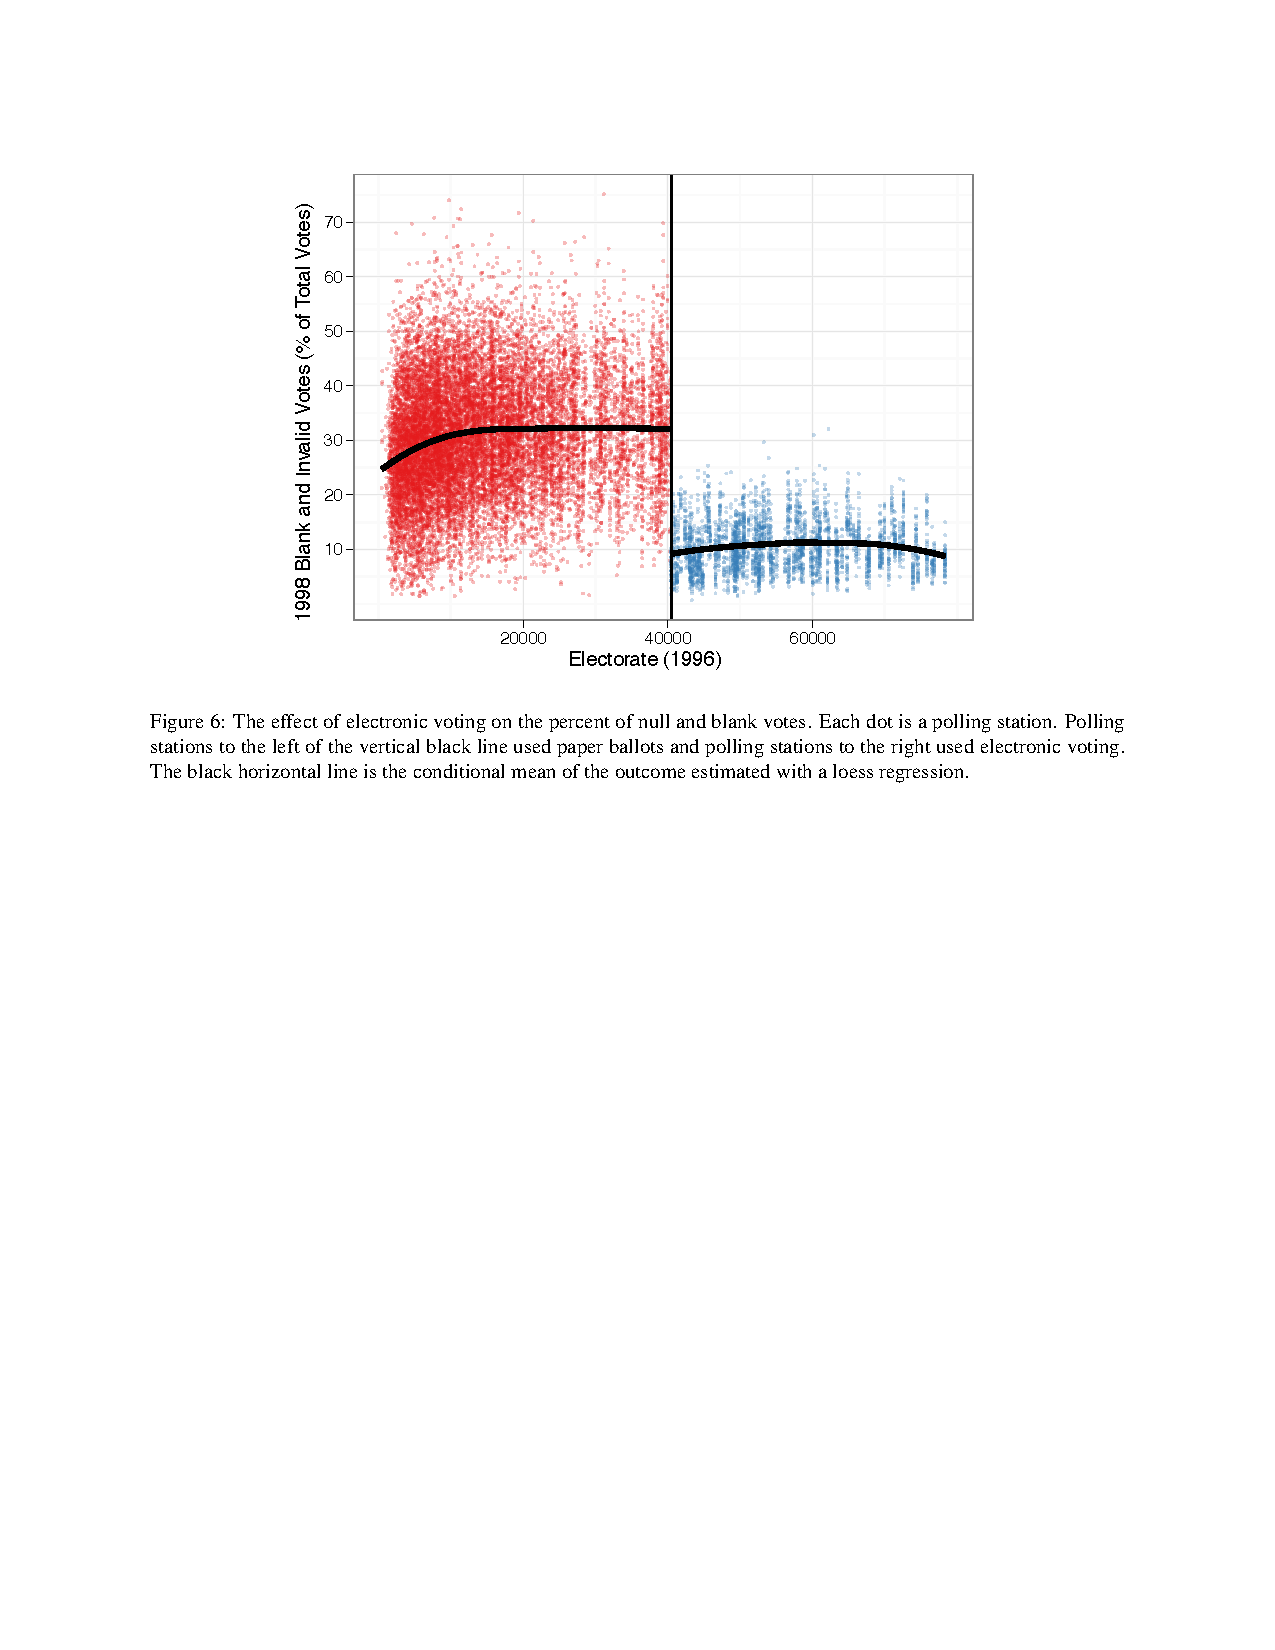
\includegraphics[height=2.9in,keepaspectratio=1]{Hidalgo1.pdf}
\end{center}
% \vspace{-.1in}
% \onslide<2-> A jump at the cutoff in the share of valid votes.
\end{frame}




%% =====================================================================
\section{The RD idea}
%% =====================================================================

\begin{frame}{Generalizing the idea}
\small
\onslide<1-> A binary treatment $D_i$ that is \textbf{determined} by whether a continuous predictor $X_i$ crosses a fixed threshold $c$:
\[
D_i = \mathbbm{1}\{X_i > c\}
\quad \Longleftrightarrow \quad
D_i = \begin{cases} 1 & \text{if } X_i > c \\ 0 & \text{if } X_i \leq c \end{cases}
\]
\onslide<2-> This is common in rule-based settings: administrative programs, eligibility cutoffs, electoral rules, age cutoffs...\\
\medskip

\onslide<3-> $X_i$: the \textcolor{Blue}{forcing} or \textcolor{Blue}{running} variable; $c$: the \textcolor{Blue}{cutoff} or \textcolor{Blue}{threshold}. \\ \medskip

\onslide<4-> $X_i$ may be (and usually is) correlated with the potential outcomes. This isn't an experiment.\\ \medskip

\onslide<5-> Later: \textit{fuzzy} RD, where $X_i > c$ \textbf{shifts the probability} of $D$ rather than determining it.
\end{frame}


% \begin{frame}{Sharp RD: graphical illustration}
% \vspace{-.3in}
% \begin{center}
%   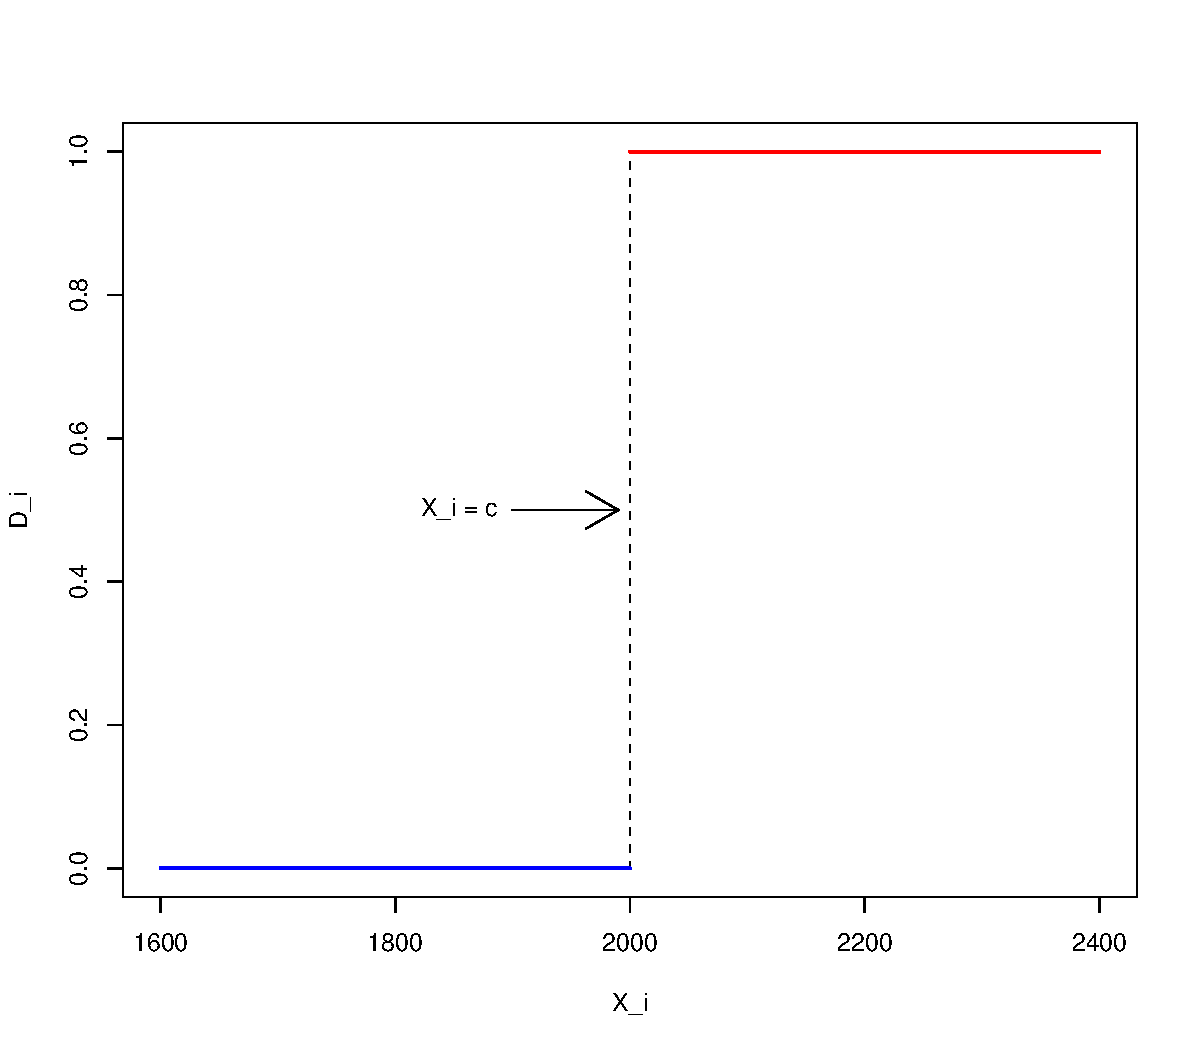
\includegraphics[scale=.4]{R1.pdf}
% \end{center}
% \end{frame}

% \begin{frame}{Sharp RD: graphical illustration}
% \vspace{-.3in}
% \begin{center}
%   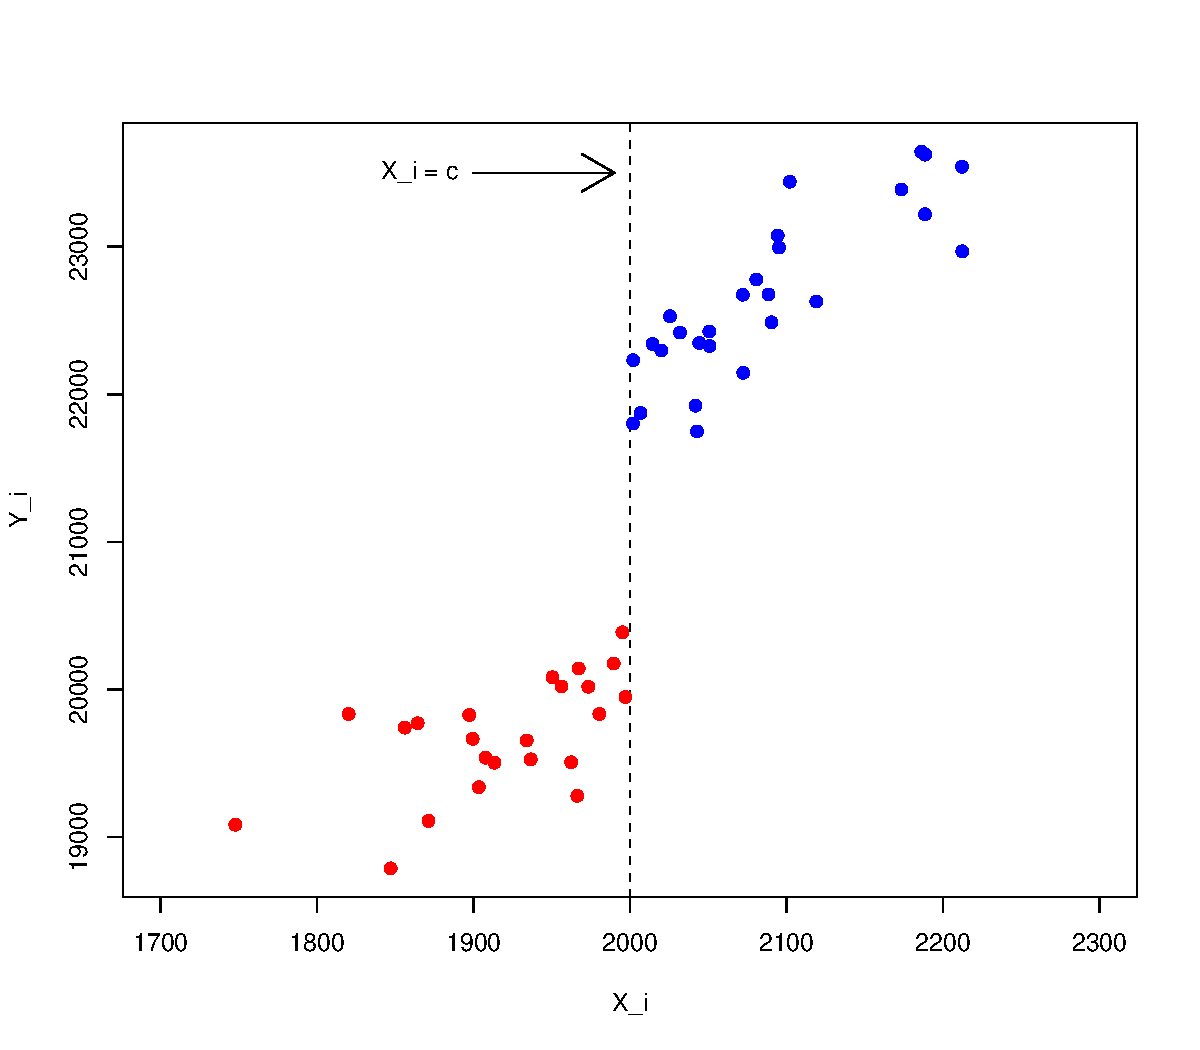
\includegraphics[scale=.4]{R2.pdf}
% \end{center}
% \end{frame}


%% =====================================================================
\section{Identification}
%% =====================================================================

\begin{frame}{Continuity of potential outcomes}
\onslide<1-> Each municipality has two potential outcomes: $Y(0)$ if paper, $Y(1)$ if e-voting, but we see only one or the other. \\
\vspace{-.05in}
\begin{center}
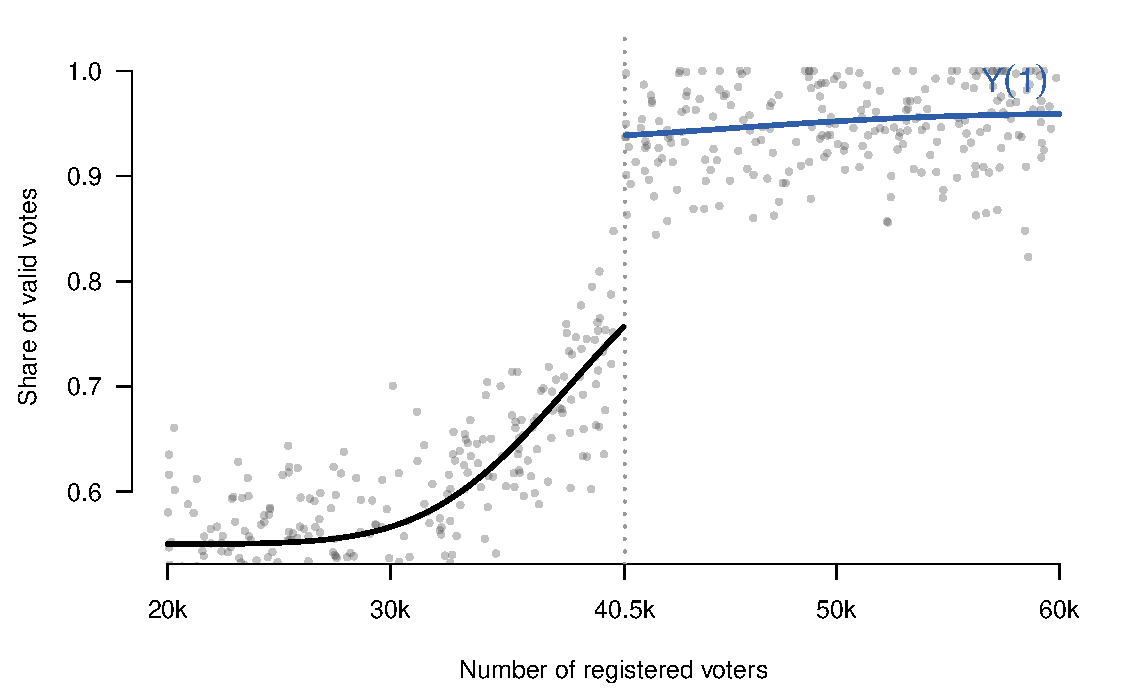
\includegraphics[height=2.4in,keepaspectratio=1]{Hidalgo_pos_2.pdf}%
%\only<3>{\includegraphics[height=2.45in,keepaspectratio=1]{Hidalgo_pos_3.pdf}}%
%\only<4->{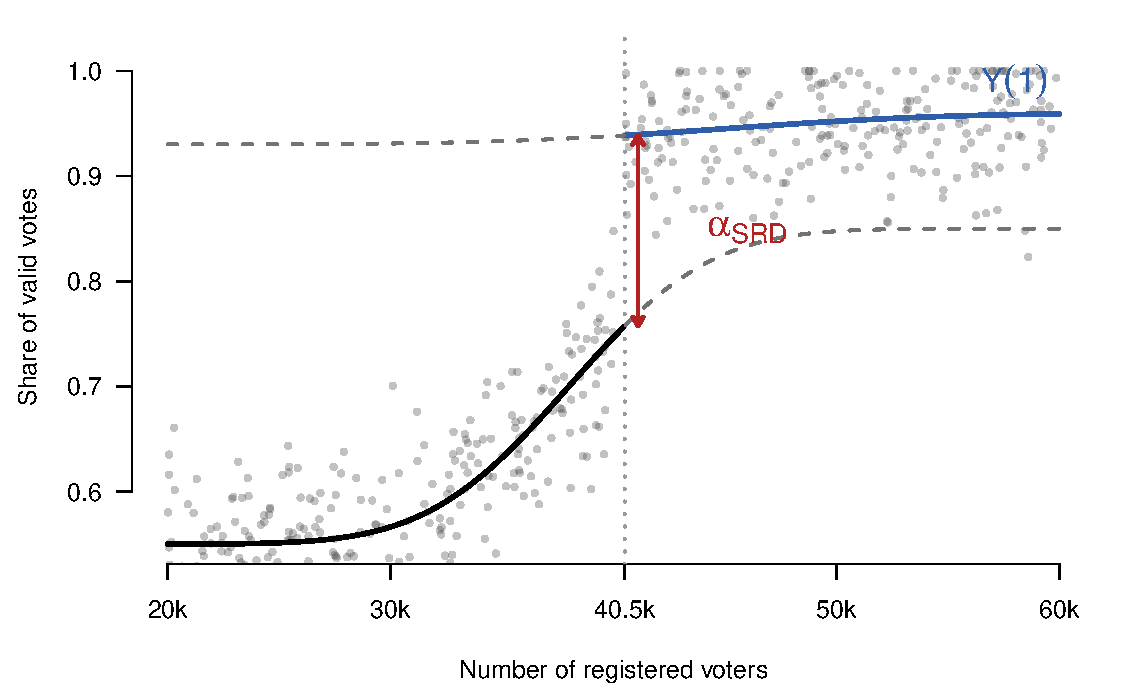
\includegraphics[height=2.45in,keepaspectratio=1]{Hidalgo_pos_4.pdf}}%
\end{center}
\end{frame}

\begin{frame}{Continuity of potential outcomes}
  \small
  \onslide<1-> Really, think of this in terms of two objects: $\E[Y(0)\mid X]$ and $\E[Y(1) \mid X]$:
\vspace{-.05in}
\begin{center}
%\only<1>{\includegraphics[height=2.45in,keepaspectratio=1]{Hidalgo_pos_1.pdf}}%
%\only<2>{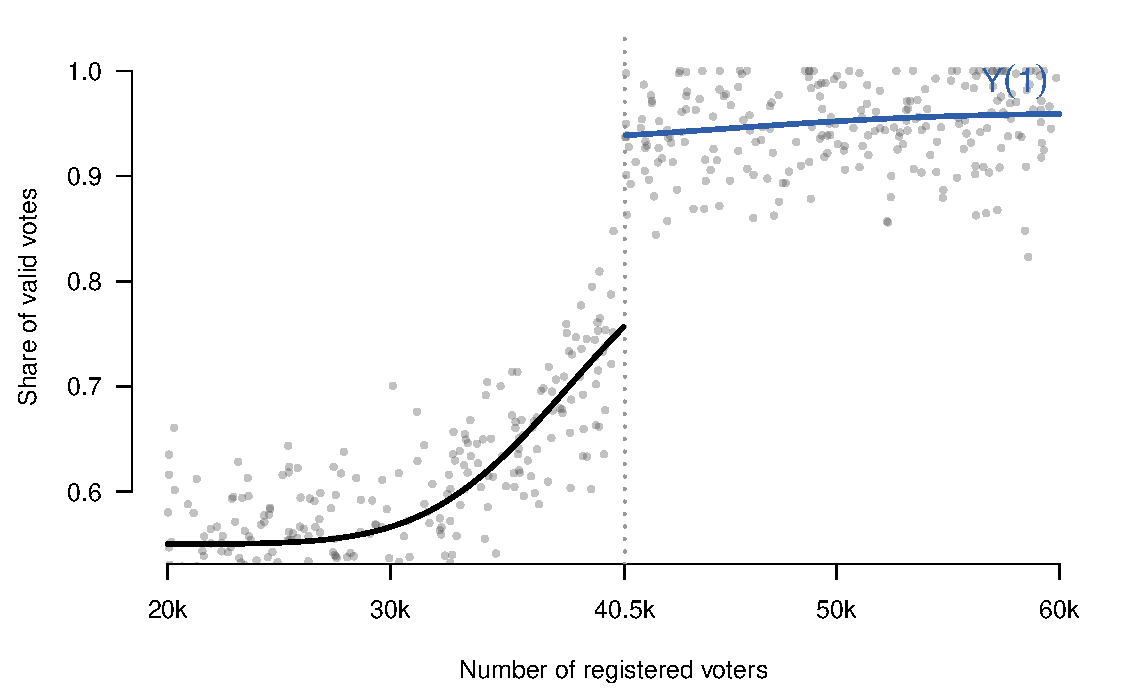
\includegraphics[height=2.45in,keepaspectratio=1]{Hidalgo_pos_2.pdf}}%
%\only<3>{\includegraphics[height=2.45in,keepaspectratio=1]{Hidalgo_pos_3.pdf}}%
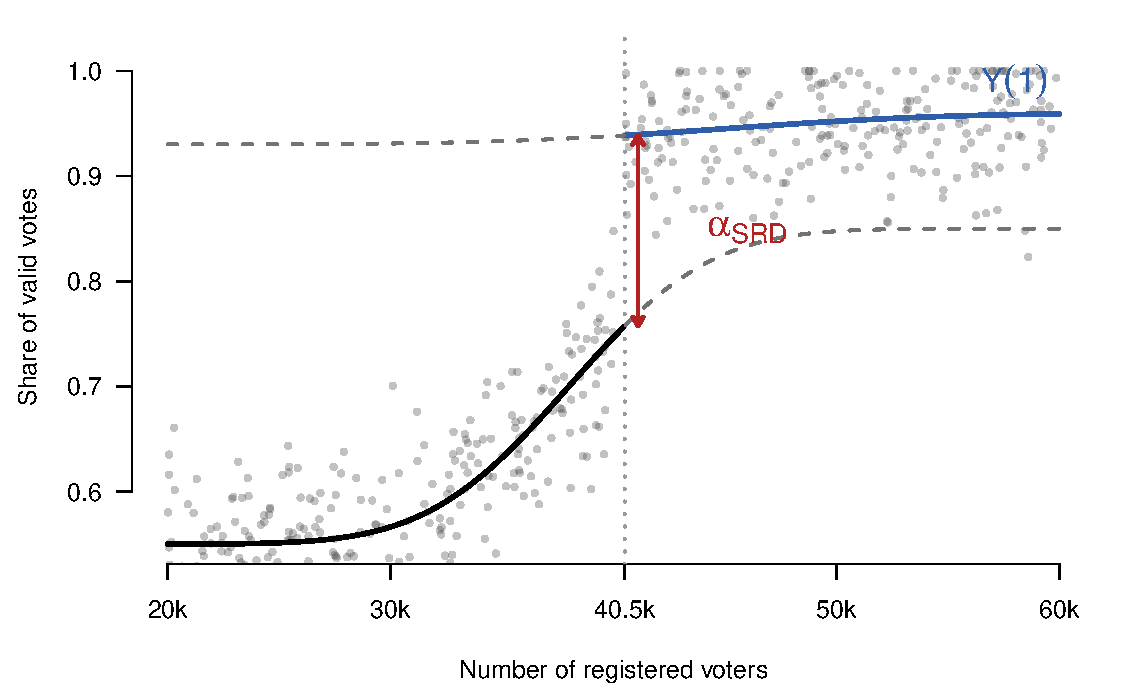
\includegraphics[height=2in,keepaspectratio=1]{Hidalgo_pos_4.pdf}%
\end{center}
\vspace{-.1in}
\small
\onslide<3-> The effect $\alpha_{SRD}$ is the vertical gap between the tracks \textit{at the cutoff}.\\
\smallskip
\onslide<4-> The core assumption is \textbf{continuity}: both tracks vary \textit{smoothly} with $X$ at $c$.
\end{frame}



\begin{frame}{Sharp RD: identification}
\onslide<1->
\begin{iass}[Continuity of conditional expectations]
$\E[Y_{1i} \mid X_i]$ and $\E[Y_{0i} \mid X_i]$ are continuous in $X_i$ at $X_i = c$.
\end{iass}
\medskip
\onslide<2-> \textcolor{Blue}{Plain-language}: Both potential outcomes CEFs move \textit{smoothly} across the running variable, at least at the cutoff.
\medskip

\onslide<3->
\begin{ires}
The treatment effect at the threshold is identified as:
\begin{eqnarray*}
\alpha_{SRD} &=& \E[Y_{1i} - Y_{0i} \mid X_i = c] \\
 &=& \lim_{x \downarrow c} \E[Y_i \mid X_i = x] \;-\; \lim_{x \uparrow c} \E[Y_i \mid X_i = x]
\end{eqnarray*}
Without further assumptions, $\alpha_{SRD}$ is \textbf{only valid at the threshold}.
\end{ires}
\end{frame}


\begin{frame}{Comments on identification}
\small
\begin{itemize}
\item<1-> We are only saying that $Y(0)$ and $Y(1)$ don't suddenly \textit{jump} at $X=c$.
\medskip
\begin{itemize}
\item<2-> We are \textit{not} saying $Y(0)$ and $Y(1)$ are unrelated to $X$, 
\item<3-> We are \textit{not} saying $Y(0)$ and $Y(1)$ are flat or have the same shape.
\end{itemize}
\medskip
\item<4-> \textcolor{Blue}{The main thing that would violate this:} another treatment kicking in at the same cutoff.
\begin{itemize}
\footnotesize
  \item If something else changes at $X=c$ that affects $Y$, then even $Y(0)$ (and $Y(1)$) jump -- i.e. a discontinuity.
  \item Plainly, RD would mis-attribute the effect of another treatment to the one you are thinking about.
\end{itemize}
\medskip
\end{itemize}
\normalsize
\begin{center} 
  \onslide<5-> This is \textit{the main} threat to keep in mind. We'll return to it.
\end{center}
\end{frame}


%% =====================================================================
\section{More examples}
%% =====================================================================

\begin{frame}{Duverger's Law (Eggers, 2010)}
\small
\begin{itemize}
\item<1-> \textbf{Duverger (1972)}: ``a majority vote on one ballot is conducive to a two-party system; proportional representation is conducive to a multiparty system.'' \medskip
\item<2-> Prediction: more parties under PR than under FPTP. \medskip
\item<3-> French municipal elections use a population rule:
\begin{itemize}
  \item $<$ 3{,}500 residents $\rightarrow$ first-past-the-post
  \item $\geq$ 3{,}500 $\rightarrow$ proportional representation
\end{itemize}
\end{itemize}
\medskip
\onslide<4-> $X_i$ = population, $c$ = 3{,}500, $D_i$ = PR rule, $Y_i$ = number of parties.
\end{frame}

\begin{frame}{Duverger's Law: the jump}
\vspace{-.2in}
\begin{center}
  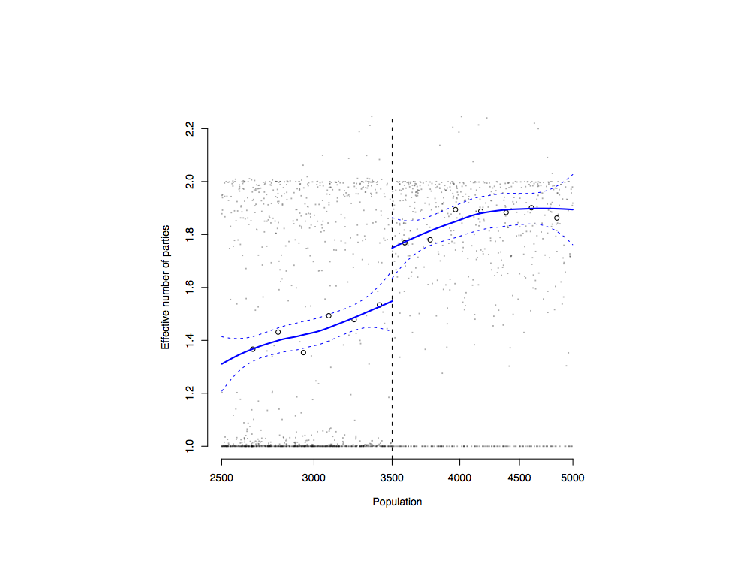
\includegraphics[height=3in,keepaspectratio=1]{egg1.pdf}
\end{center}
\end{frame}


\begin{frame}{Incumbency advantage (Lee, 2008)}
%\vspace{-.1in}
\begin{center}
  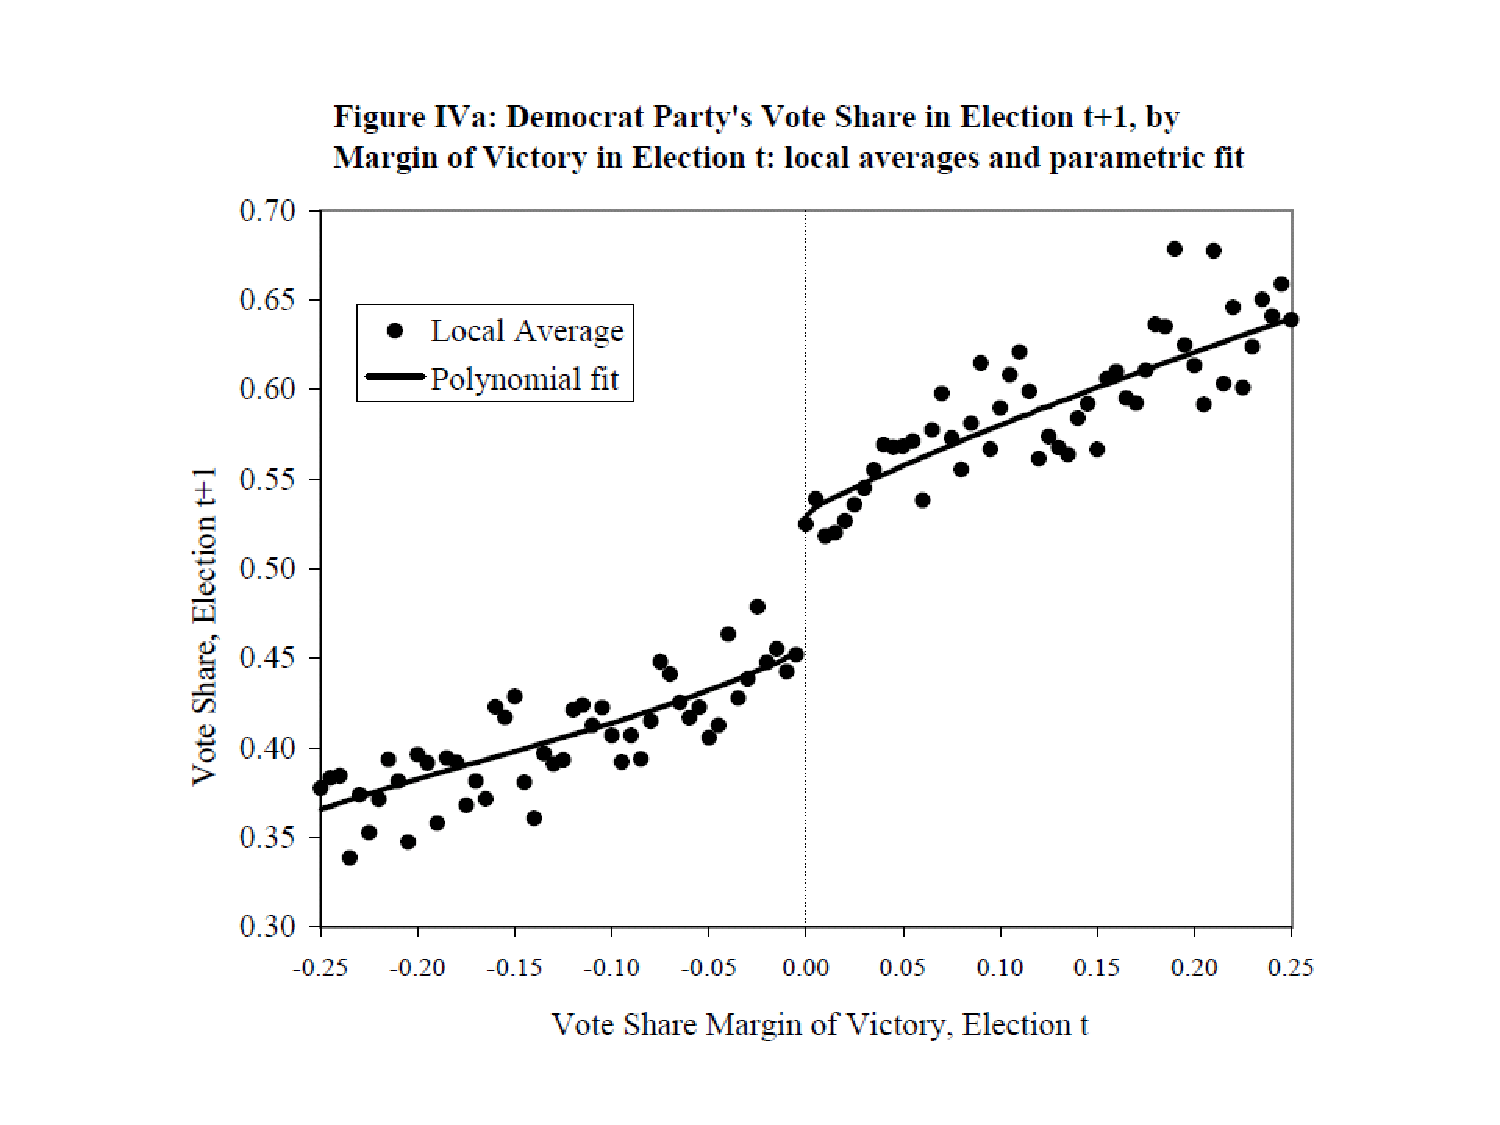
\includegraphics[height=2in,keepaspectratio=1]{lee1.pdf}
\end{center}
\small
\begin{itemize}
\item  $X_i$ = Dem party vote margin in last election, 
\item $c$ = 0, $D_i$ = won the seat, 
\item $Y_i$ = Dem party vote share next election.
\end{itemize}
\end{frame}


\begin{frame}{A few others}
\small
\begin{itemize}
\item Effect of class size on student achievement (Angrist \& Lavy 1999, Maimonides' rule)
\item Effect of access to credit (loan offer determined by credit score threshold)
\item Effect of mayoral wages on performance (Ferraz \& Finan 2011)
\item Effect of winning office on politicians' wealth (Eggers \& Hainmueller 2009)
\item Effect of school district boundaries on home values (Black 1999)
\item ``Close election'' RD has become a workhorse for electoral research: \\
  {\footnotesize Lee, Moretti \& Butler 2004; Pettersson-Lidbom 2008; Eggers \& Hainmueller 2009; many more.}
\end{itemize}
\medskip
\onslide<2-> \textcolor{Red}{Warning}: ``close election'' designs with treatment other than \textit{winning} (party, gender, education) measure the effect of \textit{electing somebody with that characteristic} -- think districts, not individuals.
\end{frame}


%% =====================================================================
\section{Estimation}
%% =====================================================================

\begin{frame}{How to actually estimate}
\small
\onslide<1-> Historically, or when casually exploring the data, you might try some simple polynomial models:
\footnotesize
\begin{itemize}
  \small
\item Choose a window of the data somewhat near the cutoff to look at.
\item Transform your $X$ to be zero at $X=c$, i.e. $\tilde{X} = X-c$.
\item Use a linear, quadratic, or cubic model plus a shift at $X=c$; better to allow different slopes on each side
\item E.g., $Y \sim  \tilde{X} + \tilde{X}^2 + D + \tilde{X}D + \tilde{X}^2 D$
\end{itemize}
\medskip
\small
\onslide<2-> But, there are important underlying estimation choices to make here that are better addressed by certain estimators.  We will discuss two.\\
\medskip
\onslide<3-> Both are local: they fit $\E[Y \mid X]$ on each side of $c$ using observations \textit{near} $c$, and read off the gap at $c$.
%\medskip
% \onslide<3-> The differences between options are mostly about:
% \begin{itemize}
%   \item how much we trust the model away from the cutoff,
%   \item how much we worry about uncertainty at the edge,
%   \item and how automated the bandwidth choice is.
% \end{itemize}
\end{frame}


\begin{frame}{Option 1: \texttt{rdrobust} (Calonico, Cattaneo, Titiunik 2014)}
\begin{center}
  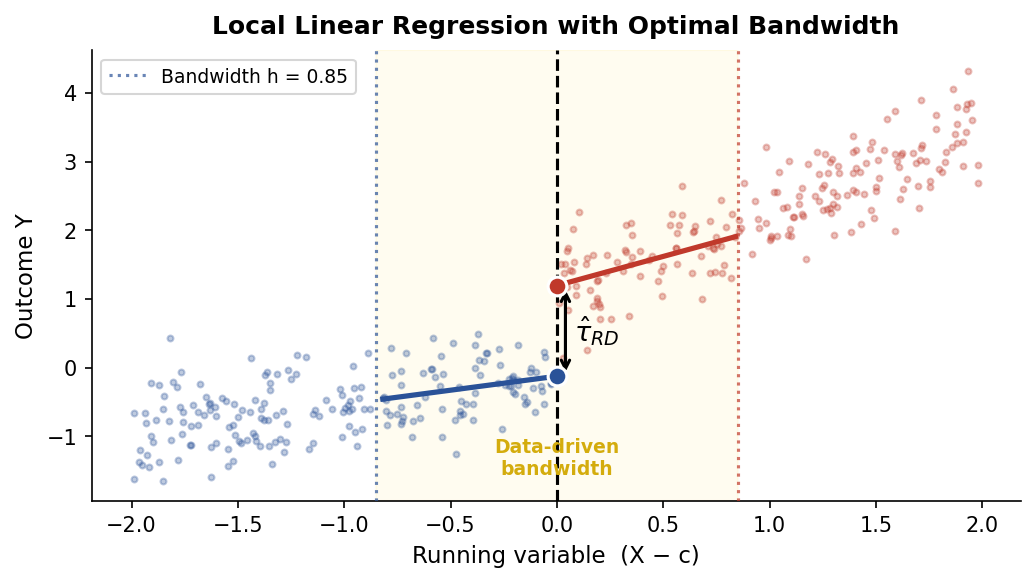
\includegraphics[scale=.45]{fig_rdrobust.png}
\end{center}
\vspace{-.05in}
\footnotesize
\begin{itemize}\setlength\itemsep{2pt}
  \item Local linear regression on each side, triangular kernel
  \item $\hat{\alpha}$ = gap in fitted values at $c$
  \item Automated, principled bandwidth selection
  \item Bias-corrected, robust CIs
\end{itemize}
\medskip
\small
\texttt{rdrobust(y, x, c = 0)}
\end{frame}


\begin{frame}{Option 2: Gaussian process (\texttt{gpss::gp\_rdd})}
\small
\onslide<1-> Two risks of any local-polynomial fit:
\begin{itemize}
  \footnotesize
  \item Polynomials happily extrapolate near the edge --- where they have least data and most leverage.
  \item Uncertainty should \textit{grow} as we approach $c$ because we have less data around those points.
\end{itemize}
\medskip
\onslide<2-> The Gaussian process:
\begin{itemize}
  \footnotesize
  \item Fits models in a flexible space of smooth functions
  \item ``Carries'' an honest range of plausible curve fits through the data $\rightarrow$ increased uncertainty towards and past edge of the data.
  \item Regularizes model on each side to avoid misreading a few noisy points as a radically different curve.
  \item Fully automated (Cho, Kim \& Hazlett 2025): \texttt{gpss::gp\_rdd(x, y, cut)} 
\end{itemize}
\end{frame}


\begin{frame}{In practice}
\small
\begin{itemize}
\item<1-> Large samples near the cutoff: \texttt{rdrobust} and GP agree.
\medskip
\item<2-> Small samples: GP gives better estimates, better coverage, fewer extreme results.
\medskip
\item<3->  Very small samples: \texttt{rdrobust} sometimes chooses very wide bandwidth or generates extreme results or NA.
\end{itemize}
\end{frame}


\begin{frame}{Random $Z$ and $Y$, large sample}
\small
\onslide<1-> $\tau \in \{0, 3\}$, $N=500$, \texttt{rdrobust} at defaults vs \texttt{gp\_rdd} at defaults.
\begin{center}
  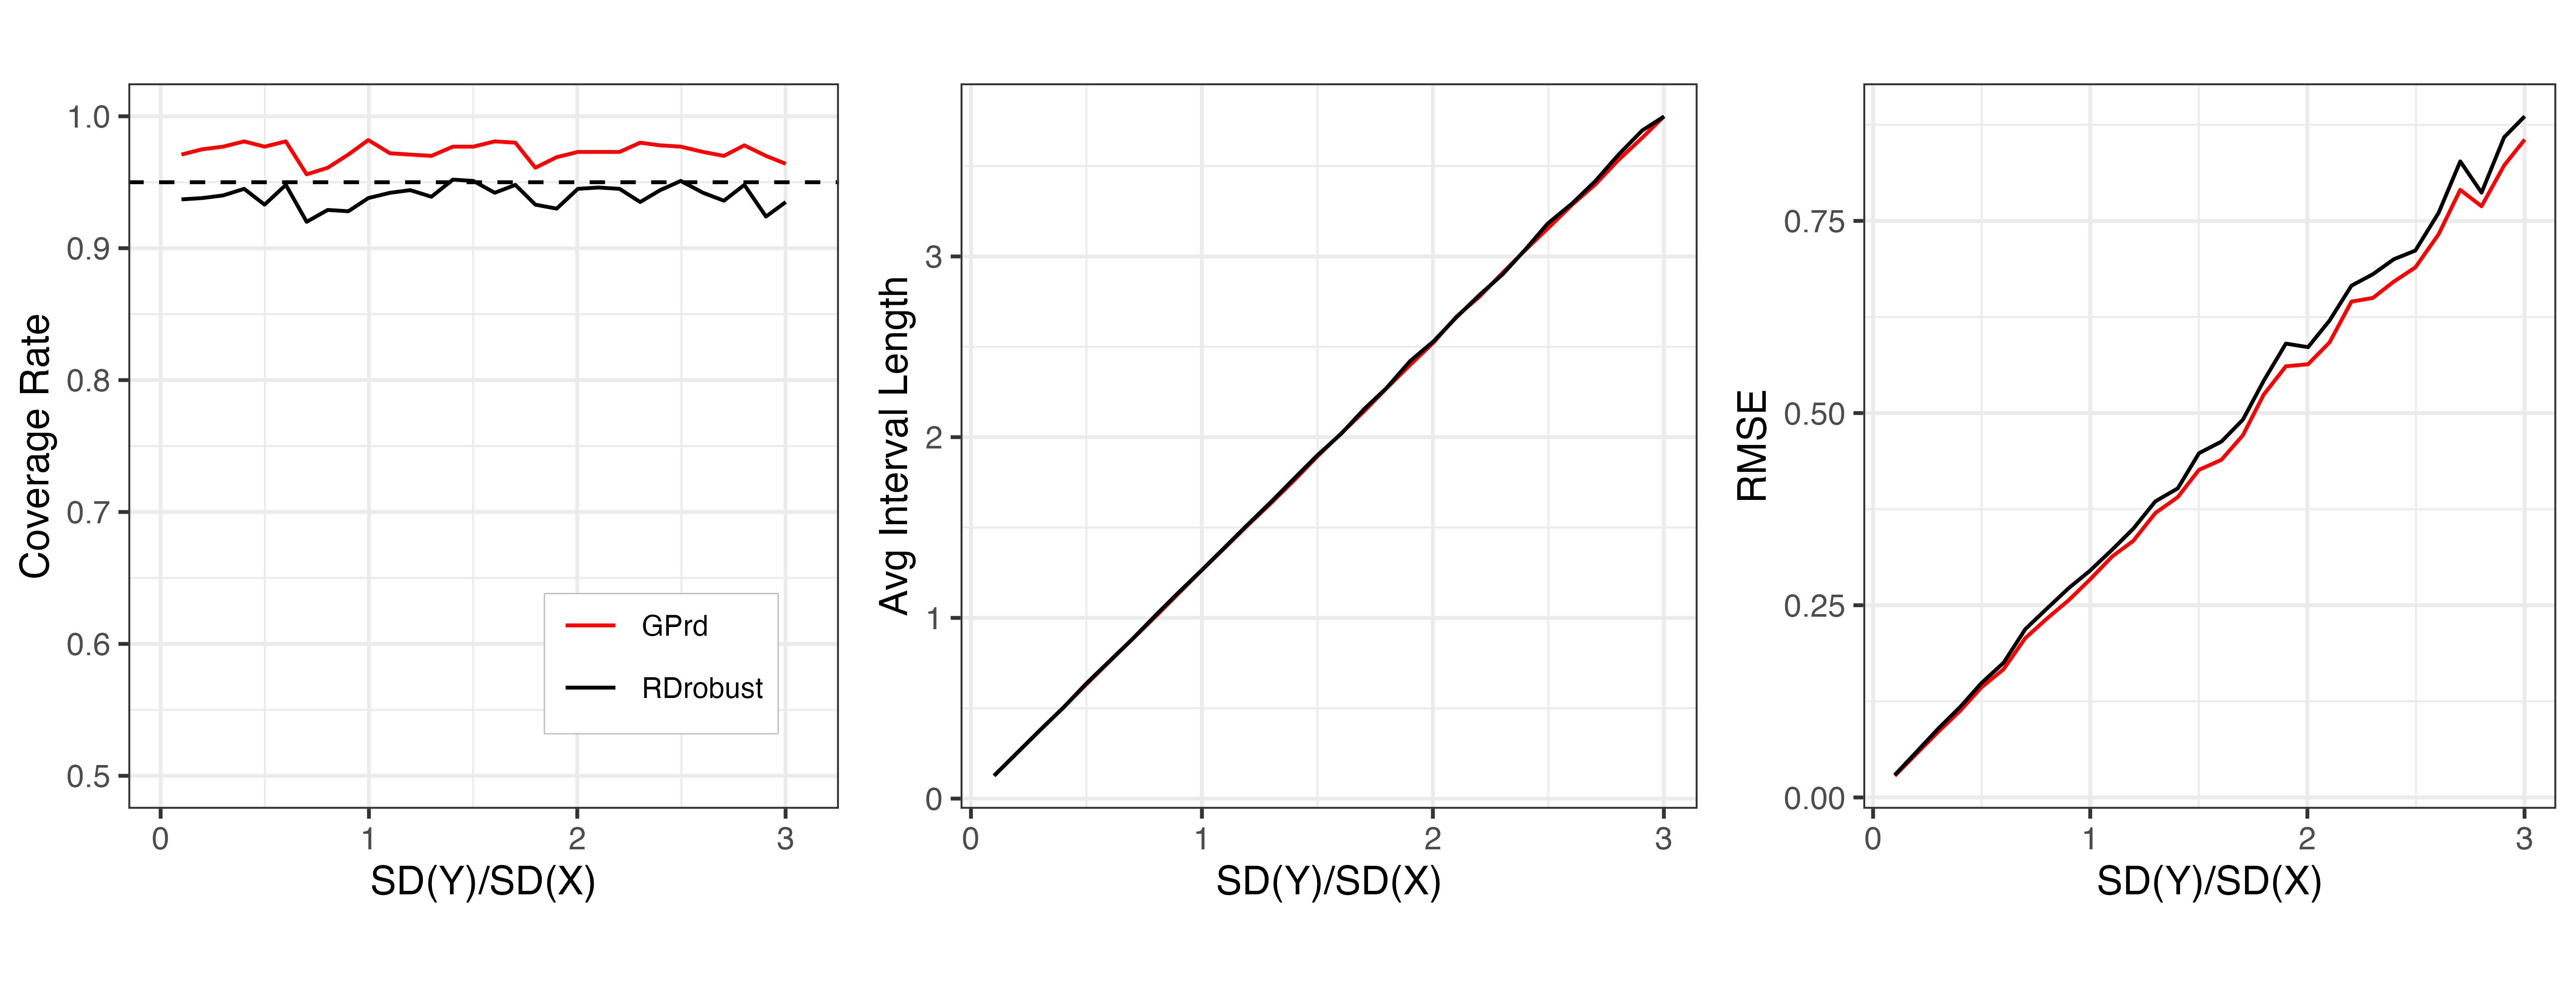
\includegraphics[width=\linewidth]{rdd_totalrandom_n500_effect0_summary.png}
\end{center}
\end{frame}


\begin{frame}{Random $Z$ and $Y$, small sample}
\small
\onslide<1-> Same DGP, $N=100$.
\begin{center}
  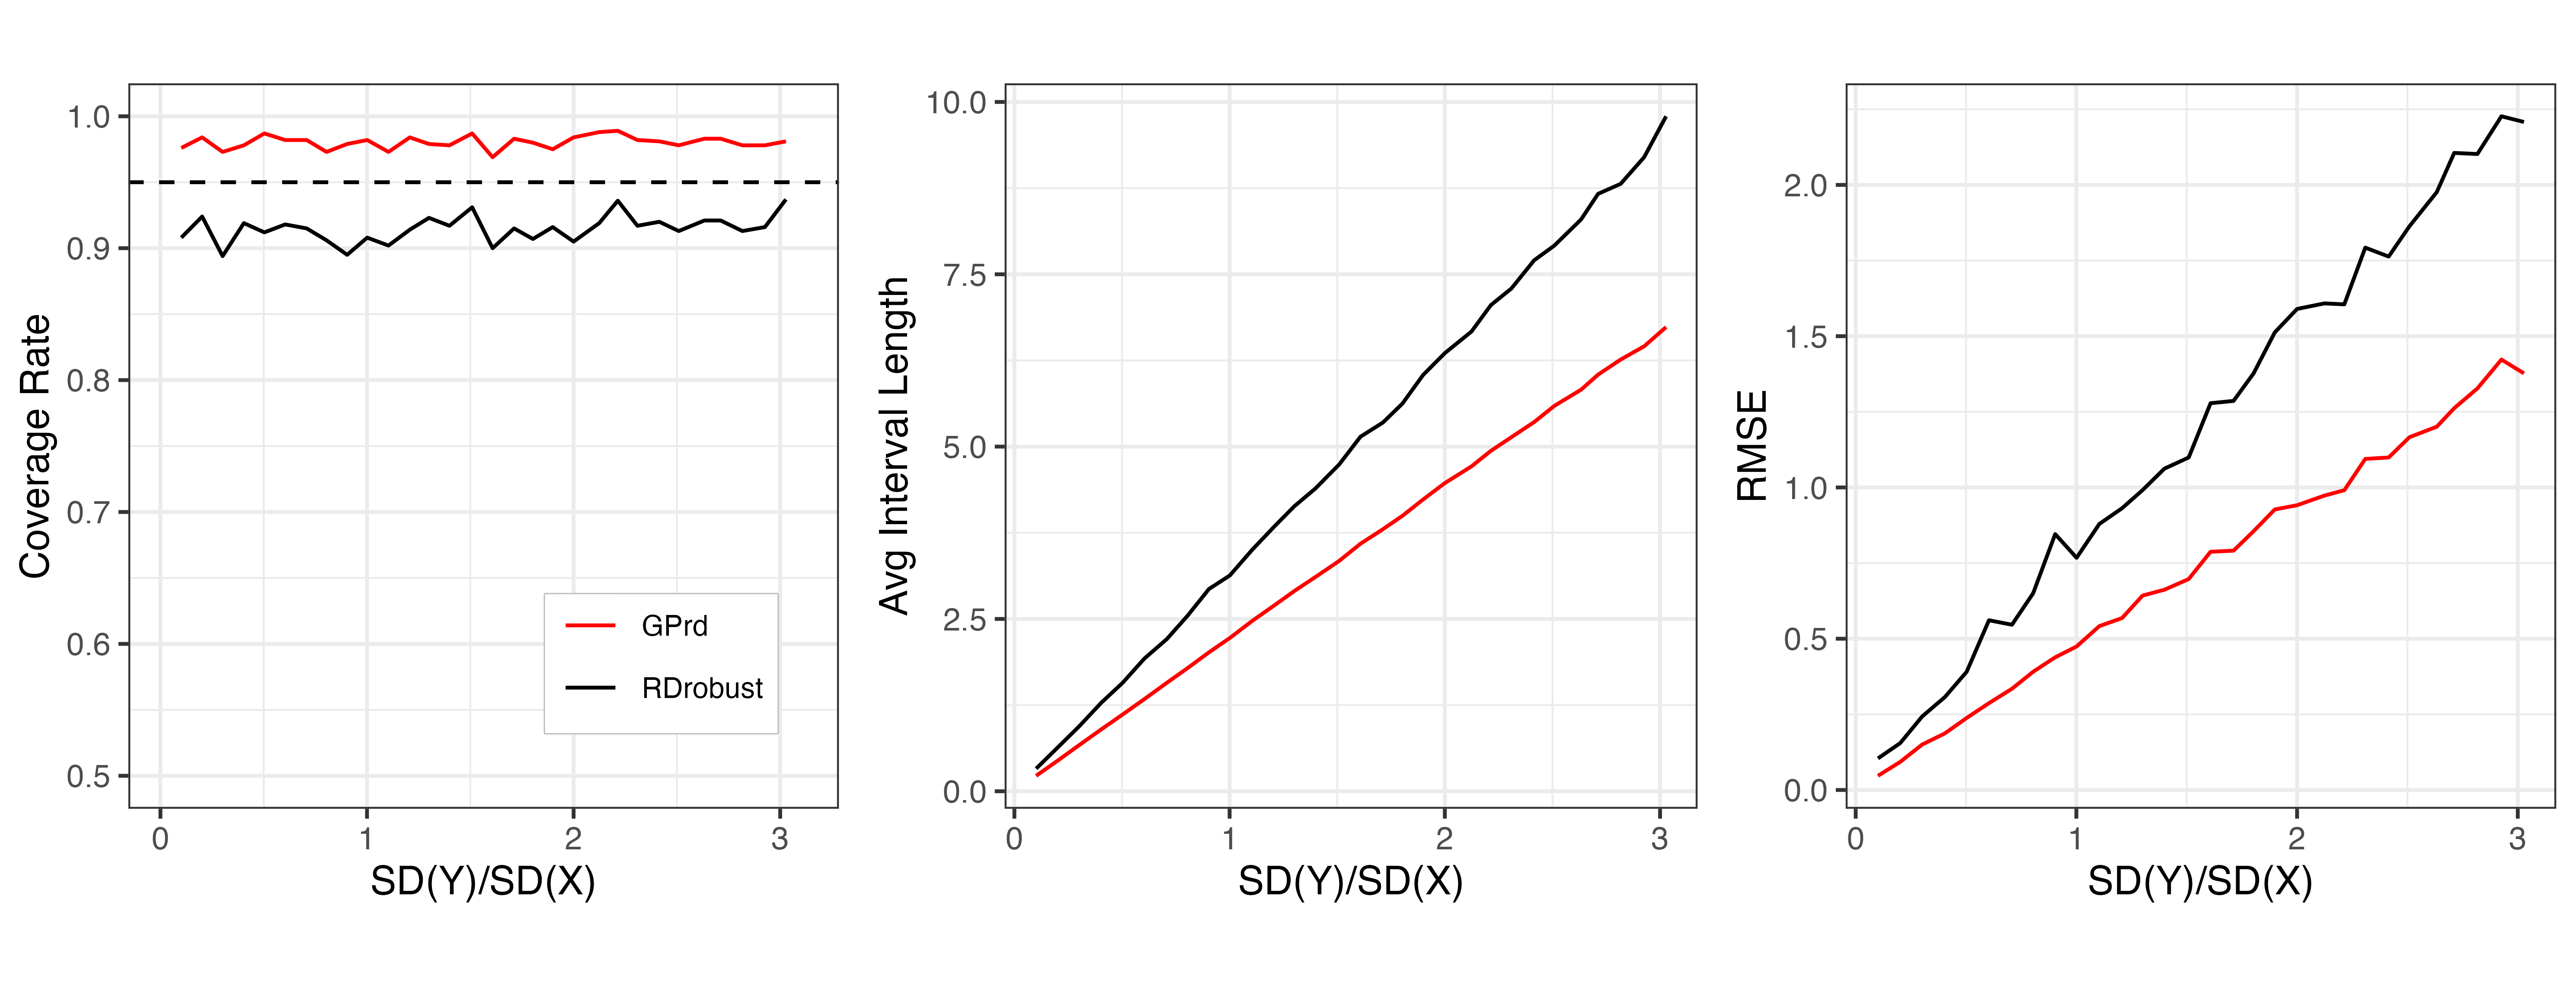
\includegraphics[width=.9\linewidth]{rdd_totalrandom_n100_effect0_summary.png}
\end{center}
\onslide<2-> Improved RMSE is the big story --- GP regularizes on each side, where polynomials can go a little crazy.
\end{frame}


\begin{frame}{Lee close elections, full sample ($N=13{,}577$)}
\small
\onslide<1-> Placebo cutoffs across Lee's close-election data. With this much data, methods barely diverge.
\begin{center}
  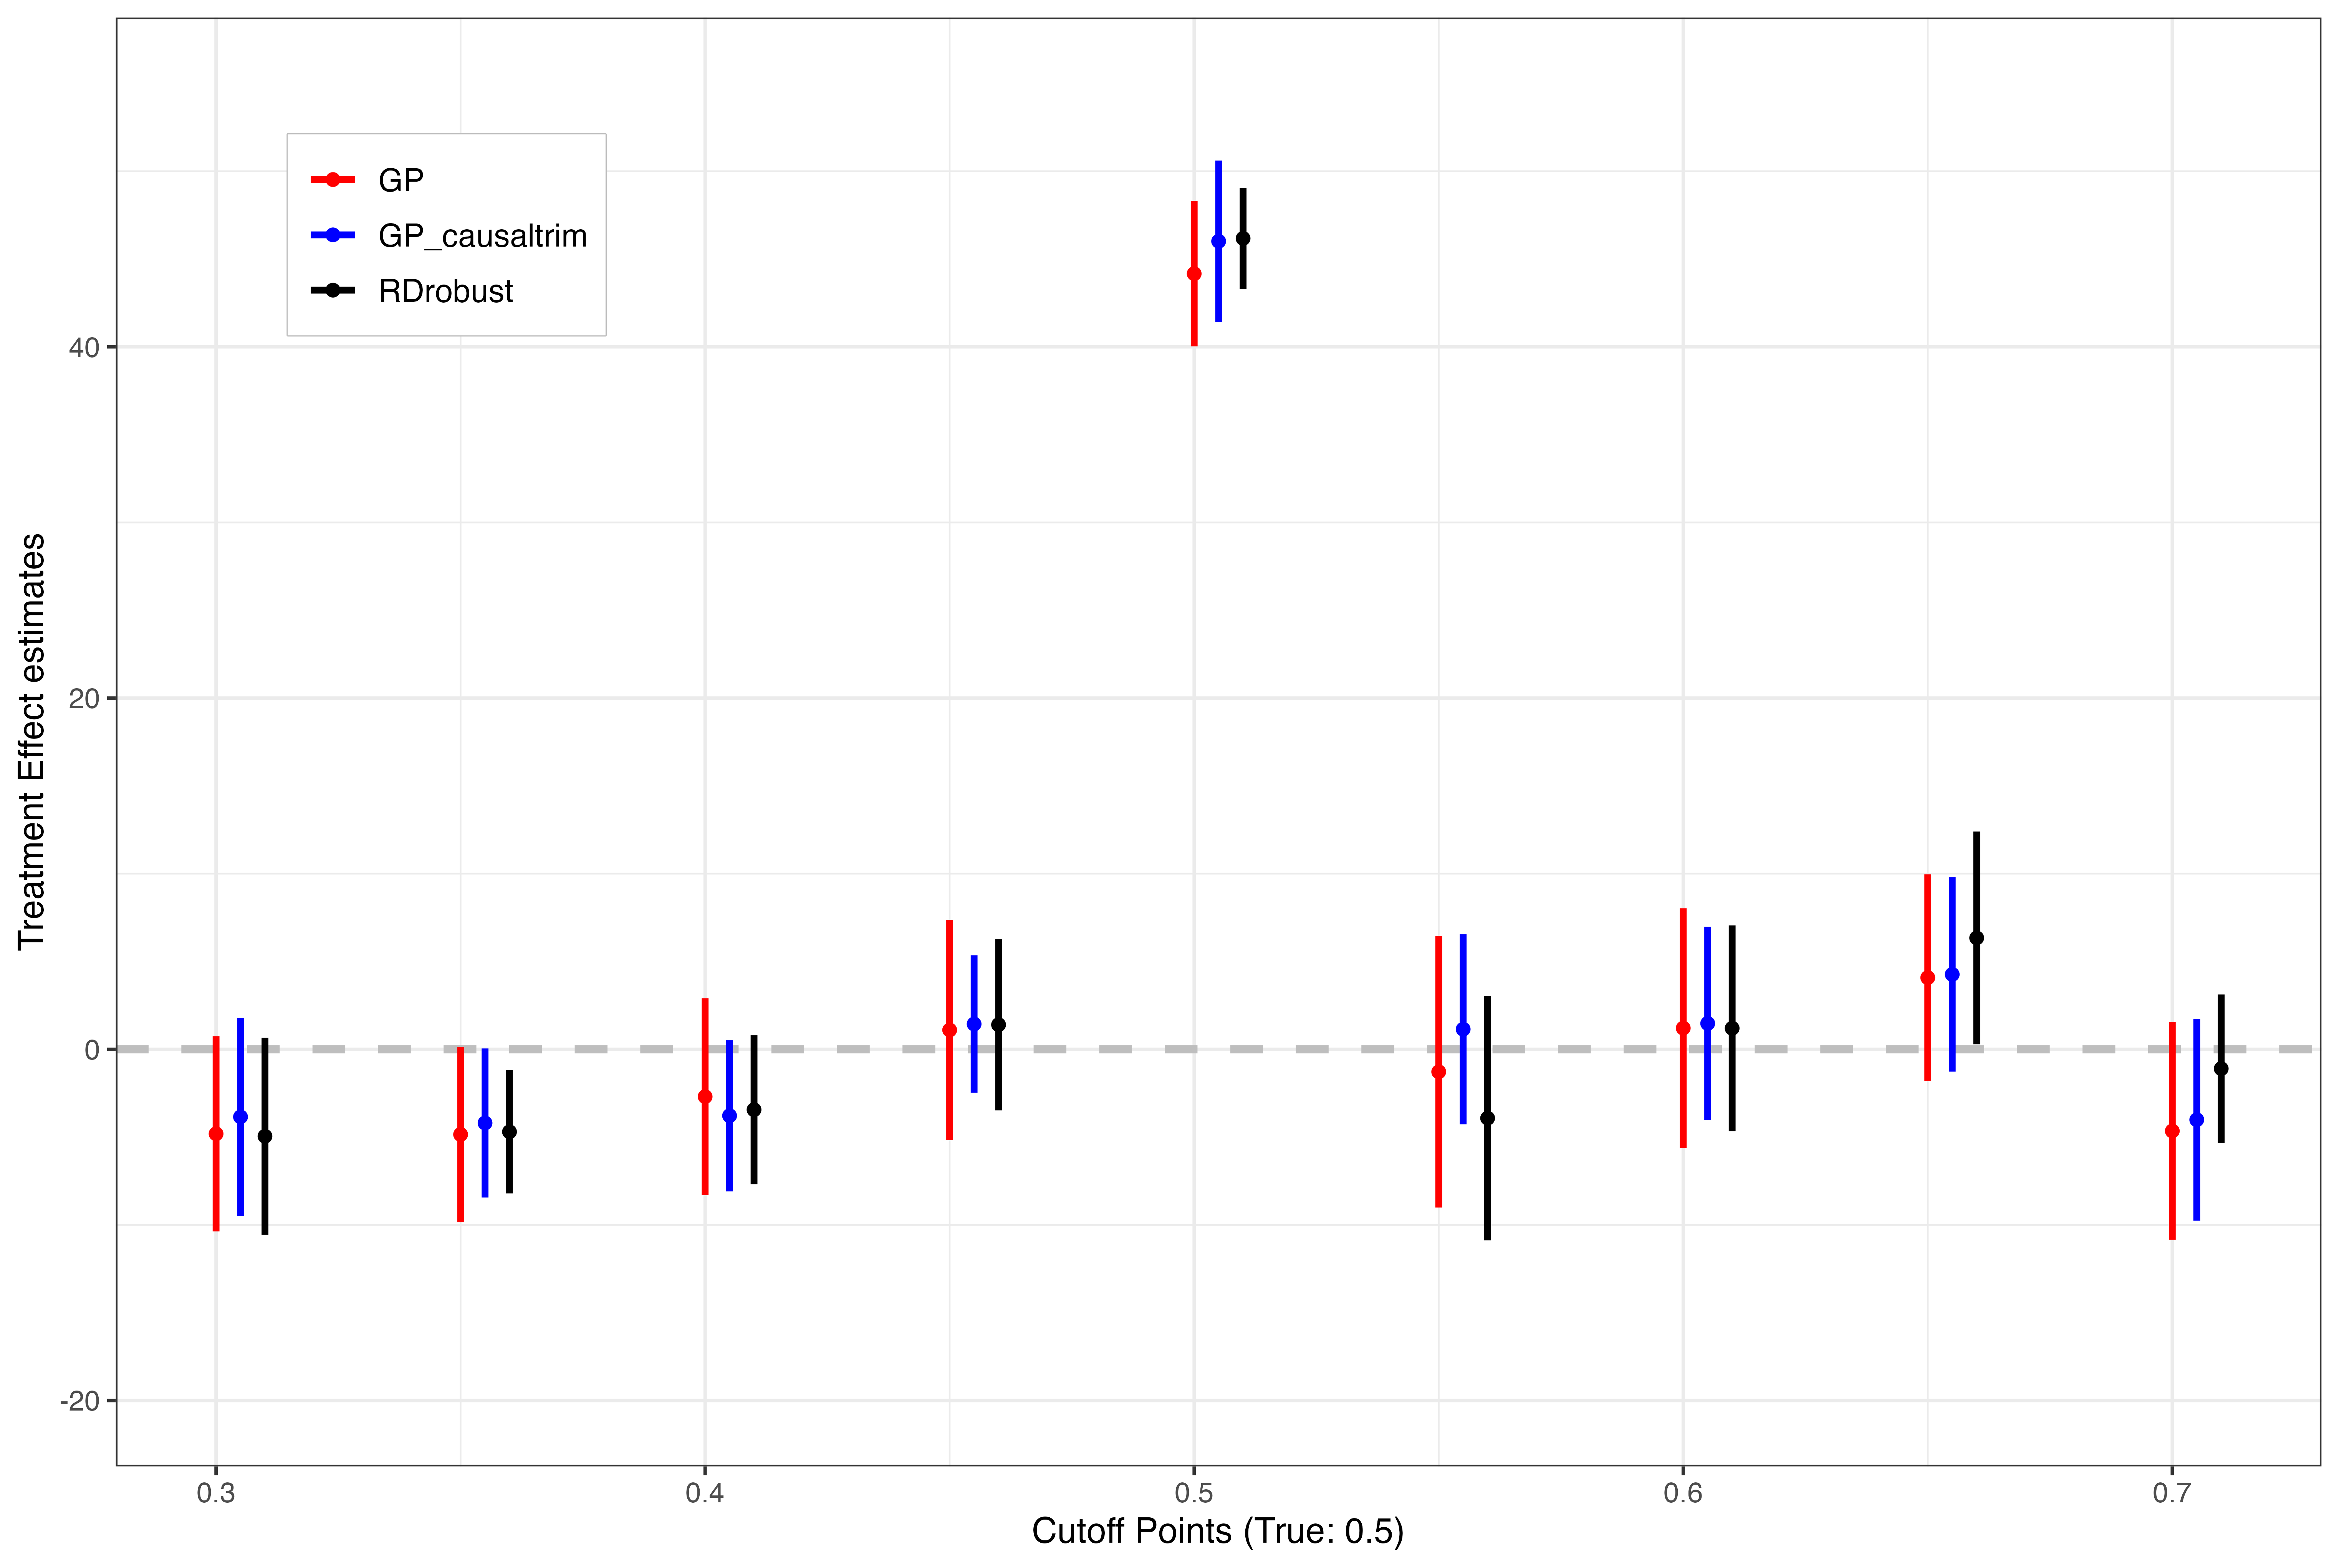
\includegraphics[width=.65\linewidth]{rdd_Lee_placebo.png}
\end{center}
\end{frame}


\begin{frame}{Lee close elections, small subsamples ($N=200$)}
\small
\onslide<1-> Repeat sampling with $N=200$ per segment. Now method choice matters.
\begin{center}
  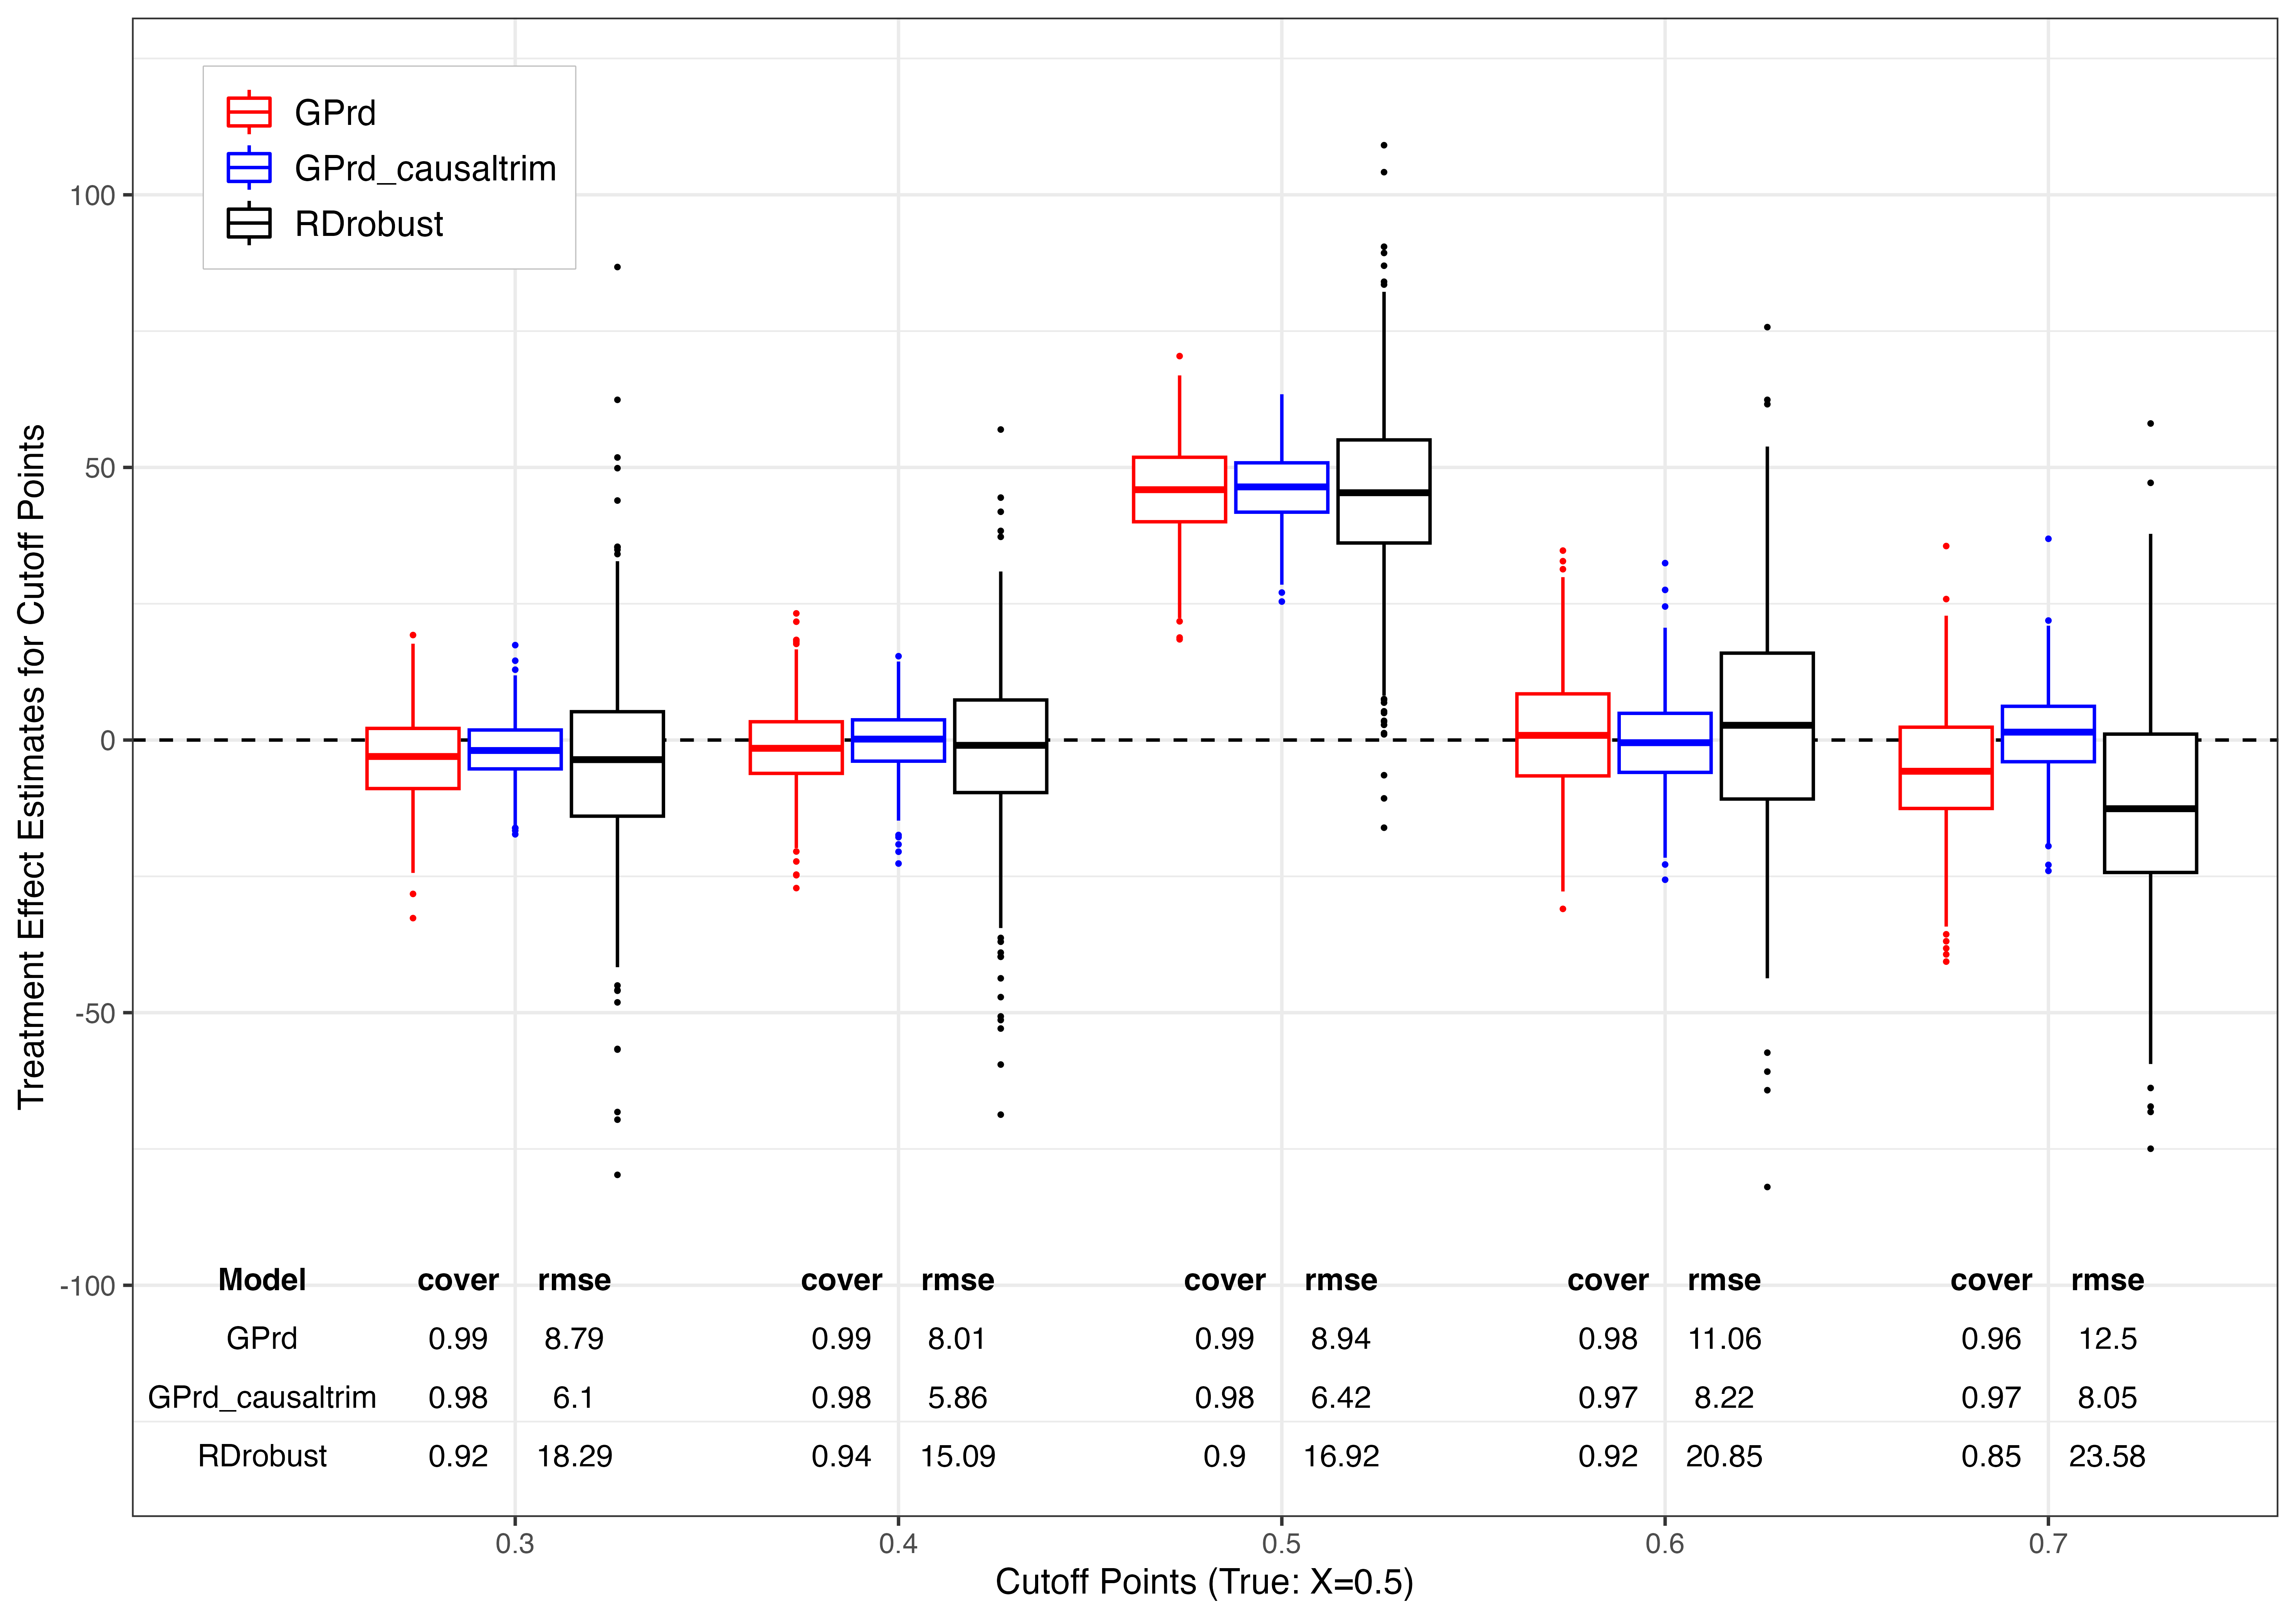
\includegraphics[scale=.42]{Figure_12_rdd_Lee_placebo_subsample_5cuts.png}
\end{center}
\end{frame}


%% =====================================================================
\section{Misspecification}
%% =====================================================================

\begin{frame}{The risk of misspecification}
\begin{center}
  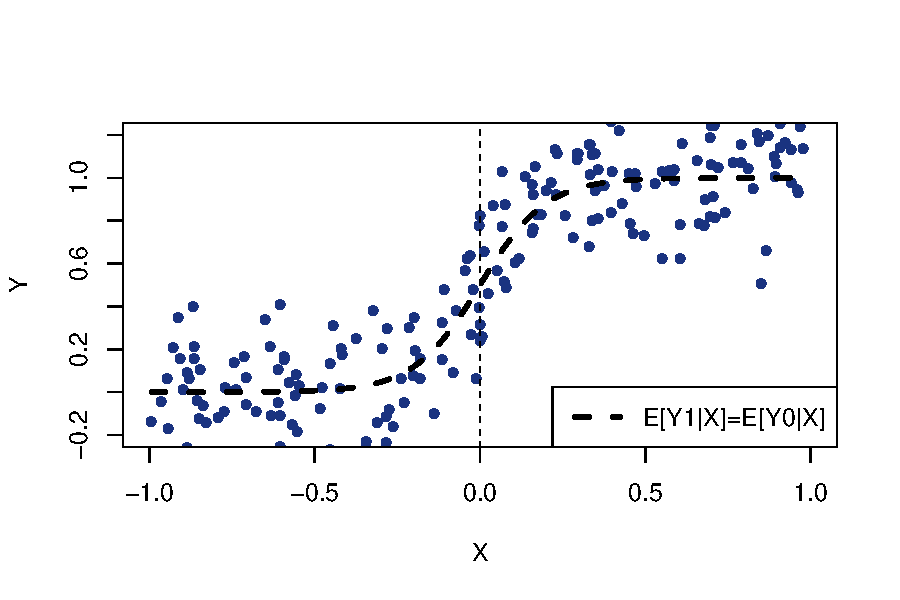
\includegraphics[scale=.7]{RDDmisspec_1.pdf}
\end{center}
\end{frame}

\begin{frame}{The risk of misspecification}
\begin{center}
  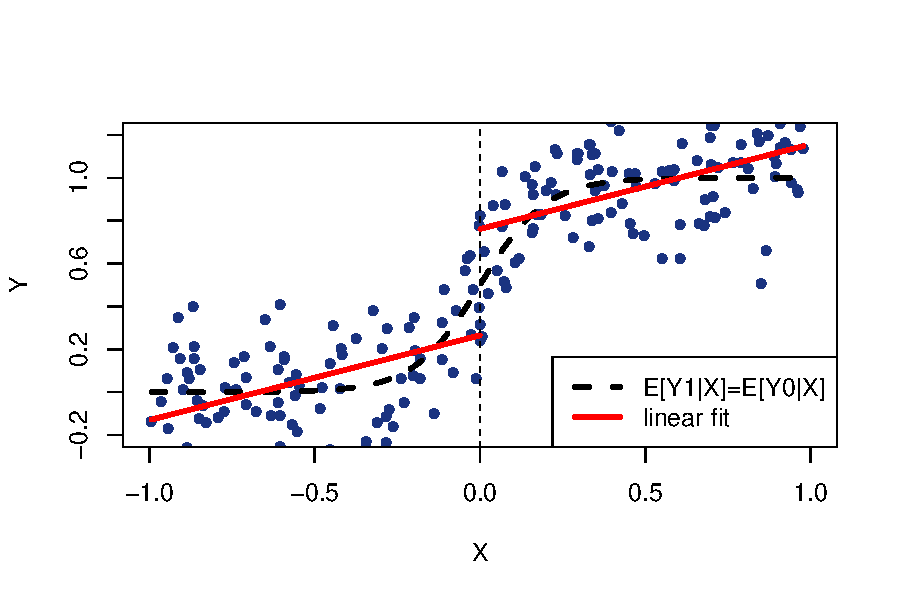
\includegraphics[scale=.7]{RDDmisspec_2.pdf}
\end{center}
\end{frame}

\begin{frame}{Same example, GP estimator}
\onslide<1-> Should be no problem at all with a suitably flexible estimator.
\begin{center}
  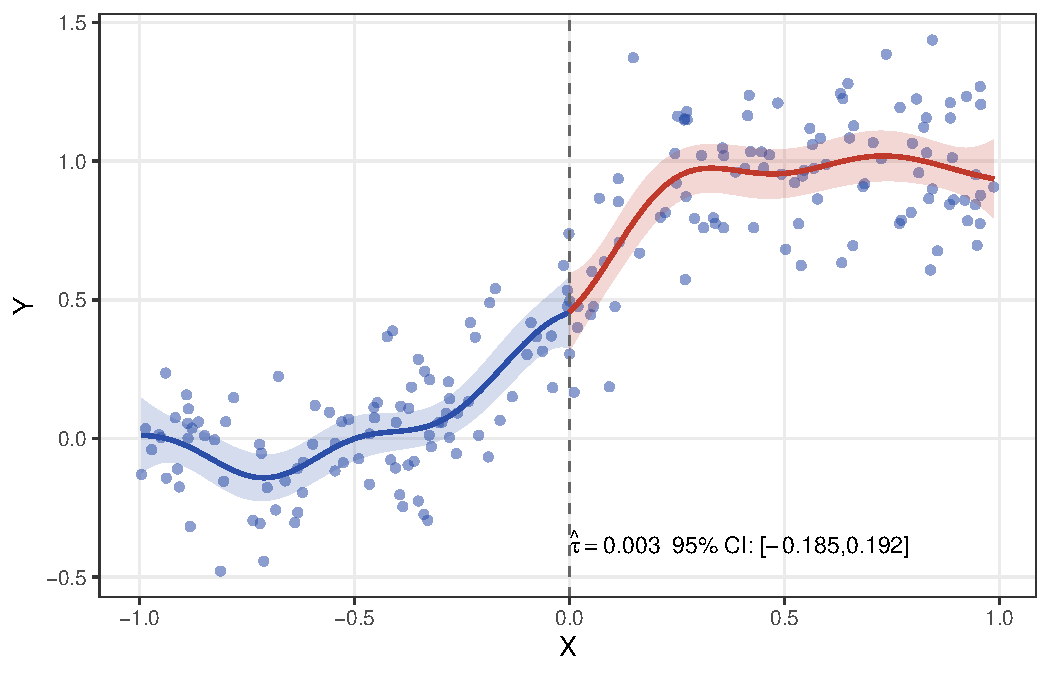
\includegraphics[scale=.5]{RDDmisspec_gprdd.pdf}
\end{center}
\onslide<2-> \texttt{gpss::gp\_rdd(x, y, cut=0)}.
\end{frame}


%% =====================================================================
\section{Falsification}
%% =====================================================================

\begin{frame}{Falsification checks: the menu}
\small
\begin{enumerate}
\item<1-> \textbf{Specification sensitivity}: are results stable across estimators / bandwidths? If not, explain. \medskip
\item<2-> \textbf{Balance}: do covariates $Z$ jump at the threshold?
\medskip
\item<3-> \textbf{Placebo outcomes}: does an outcome that \textit{shouldn't} respond to treatment also jump?
\medskip
\item<4-> \textbf{Placebo thresholds}: do you find jumps at $c^\star \neq c$?
\medskip
\item<5-> \textbf{Sorting}: do units cluster on one side of the cutoff (manipulation)?
\end{enumerate}
\end{frame}


\begin{frame}{Balance test, back to Hidalgo}
\vspace{-.1in}
\begin{center}
  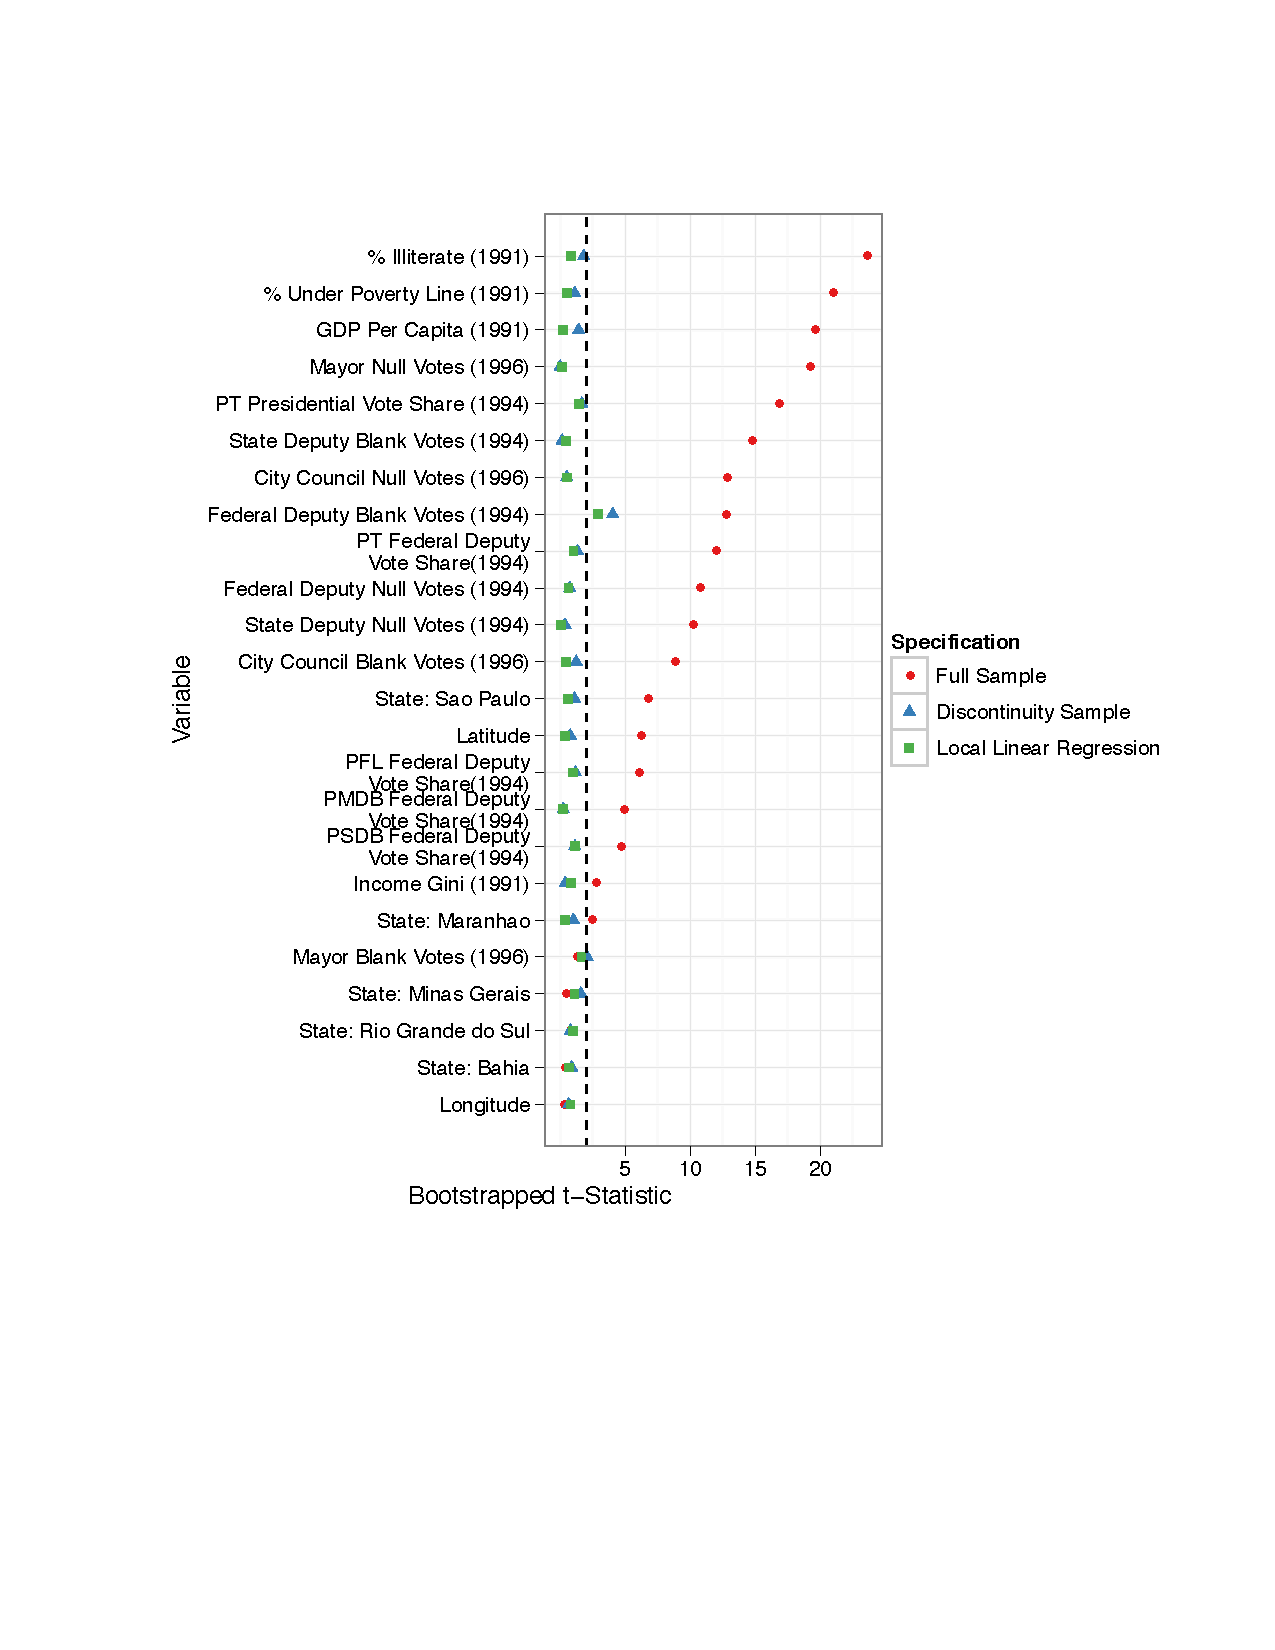
\includegraphics[height=2.7in,keepaspectratio=1]{Hidalgo2.pdf}
\end{center}
\onslide<2-> \footnotesize Run the same RD on a covariate $Z$ as the ``outcome'' --- hope for no jump.
\end{frame}


\begin{frame}{Placebo outcome (Lee 2008)}
\small
\onslide<1-> Most convincing falsification: a covariate (or pre-treatment outcome) plausibly related to potential outcomes but \textit{not} affected by treatment.
\vspace{-.05in}
\begin{center}
  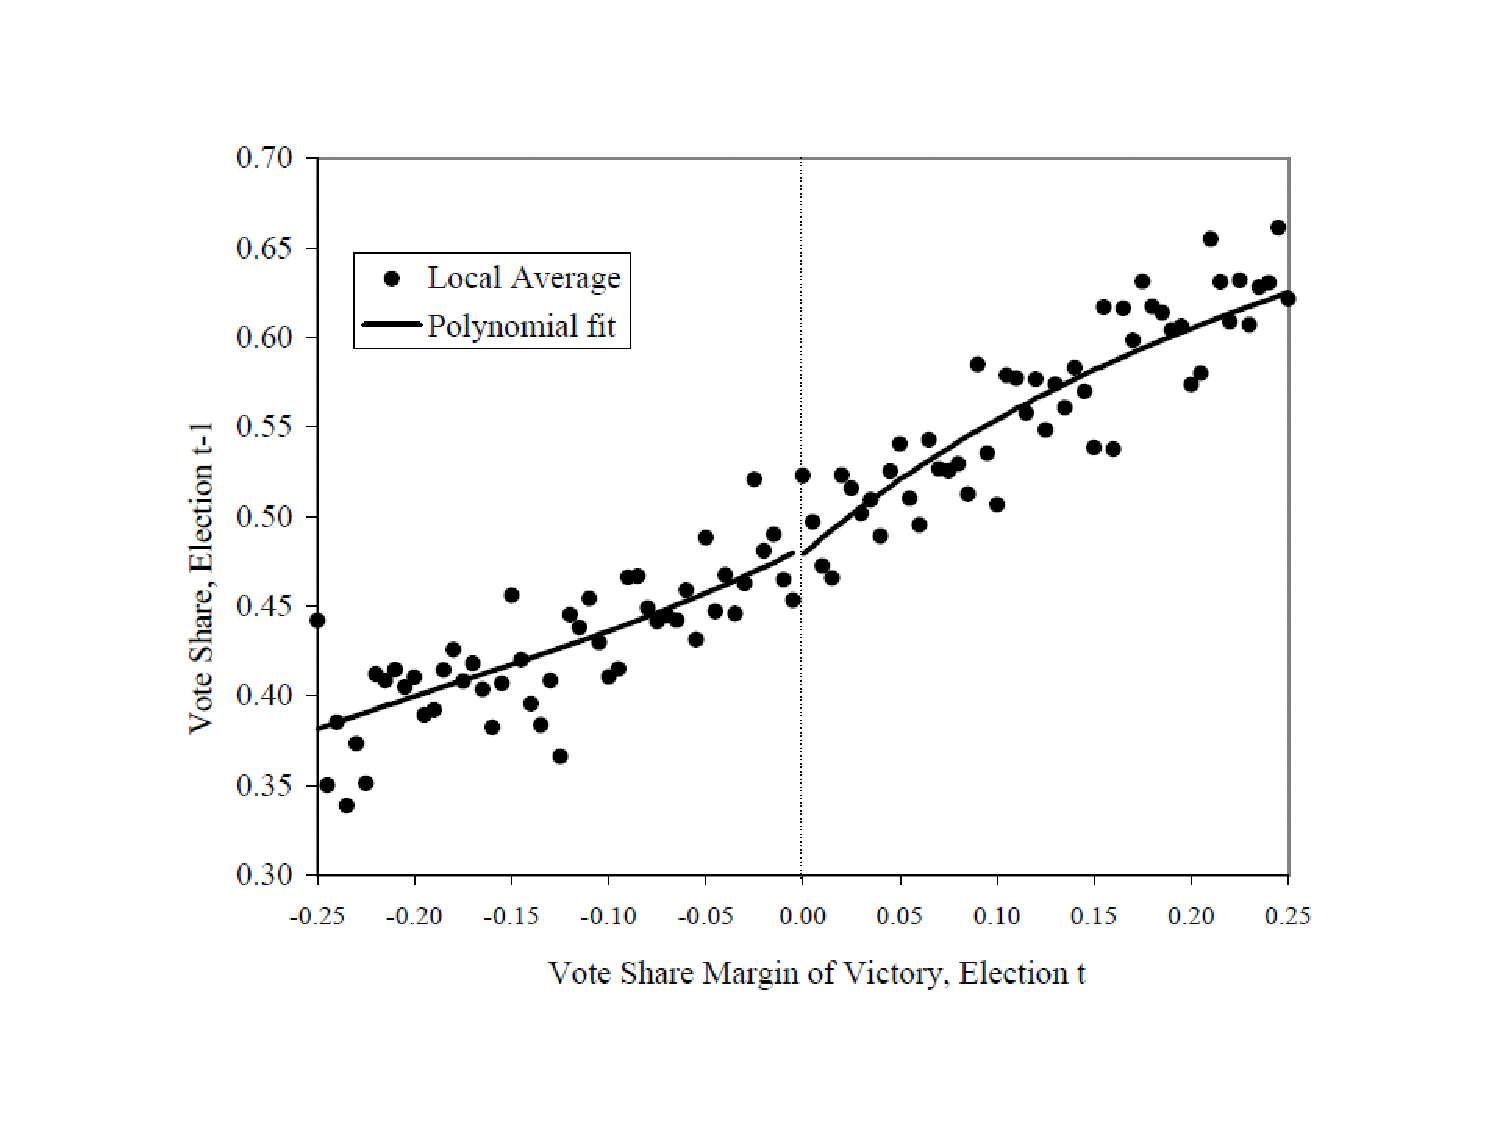
\includegraphics[height=2.5in,keepaspectratio=1]{lee2.pdf}
\end{center}
\end{frame}


\begin{frame}{Placebo thresholds and sorting}
\small
\onslide<1-> \textbf{Placebo thresholds}: pretend the cutoff is $c^\star \neq c$. Run the RD. \\
\smallskip
\begin{itemize}
  \footnotesize
  \item Detecting a jump at $c^\star$ demands an explanation.
  \item ...Are there other treatments at $c^\star$? Some reason for non-smoothness?
\end{itemize}
\bigskip
\onslide<2-> \textbf{Sorting}: can units \textit{self-select} across the cutoff?
\smallskip
\begin{itemize}
  \footnotesize
  \item Fine control over $X$ (gaming a test score, withholding income).
  \item E.g. Administrators choosing thresholds strategically.
  \item Density test (McCrary 2008): bulge in $X$ on one side of $c$?
  \item Not always a problem: sorting would have to be very precise, and widespread, to substantially bias the result.
\end{itemize}
\end{frame}


%% =====================================================================
\section{The main worry}
%% =====================================================================

\begin{frame}{The main worry: bundled treatments}
\small
\begin{itemize}
\item<1-> Sometimes \textit{multiple things} change at the same threshold.
\medskip
\item<2-> This is bad:
\begin{itemize}
  \footnotesize
  \item If a \textit{different} treatment affects $Y$ at the same cutoff then your outcome $Y$ will be hit regardless of the treatment you are asking about.
  \item That is, your $Y(0)$ and $Y(1)$ will jump at the cutoff -- violation of the continuity assumption.
  \item Essentially a confounder right at the cutoff.
\end{itemize}
\medskip
\item<3-> In other words, the RD does not tell you \textit{what} treatment effect you are seeing.
\medskip
\item<4-> \textcolor{Blue}{Always ask}: \textit{what else changes at $c$?}. This is where careful investigatory work and domain expertise pay off.
\end{itemize}
\end{frame}


%% =====================================================================
\section{Fuzzy RD}
%% =====================================================================

\begin{frame}{Fuzzy RD}
\small
\begin{itemize}
\item<1-> The threshold doesn't \textit{determine} treatment, but it \textbf{shifts the probability} of treatment.
\medskip
\item<2-> E.g.: scoring above a threshold raises the chance of getting a scholarship from 20\% to 70\%, but doesn't guarantee it.
\medskip
\item<3-> \textcolor{Blue}{This should remind you of IV.}
\smallskip
\begin{itemize}
\footnotesize
\item Crossing $c$ is the instrument.
\item It changes treatment probability and (we hope) only affects $Y$ through treatment.
\end{itemize}
\end{itemize}
\end{frame}


\begin{frame}{Doing fuzzy RD}
\small
\onslide<1-> The recipe (just like IV at the cutoff):
\begin{enumerate}
\footnotesize
  \item \textbf{Reduced form}: estimate the jump in $Y$ at the cutoff (the sharp RD on $Y$).
  \item \textbf{First stage}: estimate the jump in $D$ at the cutoff (the sharp RD on $D$).
  \item Divide.
\end{enumerate}
\medskip
\onslide<2-> \textcolor{Blue}{Toy numbers}: crossing $c$ raises income by \$5{,}000 \textit{and} raises scholarship probability from 20\% to 70\%. \\
\medskip
\onslide<3-> Compute $\hat{\alpha}_{\text{LATE}} = 5000 / 0.5 = \$10{,}000$.\\
\medskip
\onslide<4-> \textcolor{Red}{Interpretation and credibility}:
\begin{itemize}
\footnotesize
  \item The estimand is \textbf{doubly local}: at the cutoff, and only for compliers.
  \item Same threat as before: no \textit{other} treatments switching at $c$.
\end{itemize}
\medskip
\onslide<5-> \texttt{rdrobust} can do this for you (\texttt{fuzzy = D}).
\end{frame}


%% =====================================================================
\section{Wrap-up}
%% =====================================================================

\begin{frame}{Internal vs. external validity}
\small
\onslide<1-> \textcolor{Blue}{Internal validity}:
\begin{itemize}
\footnotesize
  \item Continuity of POs is often defensible, making RD one of the happiest observational approaches. 
  \item Main threat: \textbf{bundled treatments} at the same cutoff.
\end{itemize}
\medskip
\onslide<2-> \textcolor{Blue}{External validity}:
\begin{itemize}
\footnotesize
  \item You learn the average effect for units with $X_i$ \textit{near} $c$.
  \item Fuzzy RD: also restricted to compliers near $c$.
  \item No information about effects elsewhere on the $X$ distribution. Don't try.
  \item Often useful in combination with other approaches such as SOO that aim for broader target but have less credible assumptions.
\end{itemize}
\end{frame}


\begin{frame}{Takeaways}
\small
\begin{itemize}
\item<1-> RD turns an administrative rule into something close to an experiment --- locally.
\medskip
\item<2-> Identification: \textbf{continuity}. Plain English: no other (impactful) treatments at same cutoff. 
\medskip
\item<3-> Estimation: use an automated tool (\texttt{rdrobust}, \texttt{gp\_rdd})
\medskip
\item<4-> Falsification battery: balance/ placebo outcomes, placebo thresholds, sometimes sorting
\medskip
\item<5-> But most important is \textcolor{Red}{investigatory work to look for other treatments at same cutoff}.
\end{itemize}
\end{frame}

\end{document}
